\documentclass[../zhang_thesis.tex]{subfiles}
\begin{document}

\chapter{Filtering Results}

%%%%%%%%%%%%%%%%%%%%%%%%%%%%%%%%%%%%%%%%%%%%%%%%%%%%%%%%%%%%%%%

\section{Performance Measures}

The study was concerned with the accuracy and speed of the nonlinear filters on estimation of the SOC $x_1$. The accuracy was measured using the mean RMSE (MRMSE). The RMSE is defined as
\begin{equation}
    \mathrm{RMSE}(kT_s) = \sqrt{ \frac{1}{N_\text{trials}} \sum_{j=1}^{N_\text{trials}} \Big( \hat{x}_1^j(kT_s) - x_1^j(kT_s) \Big)^2 },
\end{equation}
where $T_s$ is the sample period and the superscript $j$ indicates the $j$th Monte Carlo trial. This study used $N_\text{trials}=100$ Monte Carlo trials. Then, the MRMSE is the mean of the RMSE over time, giving
\begin{equation}
    \mathrm{MRMSE} = \frac{1}{N} \sum_{k=1}^N \mathrm{RMSE}(kT_s),
\end{equation}
where $N$ is the total number of times at which the filtering was performed. An additional measure of accuracy was the number of trials in which the filter estimate diverged. A divergence is considered an absolute error in teh estimated SOC greater than $0.1$~V or any failure in the filtering process, such as due to a non-invertible matrix or a non-positive definite covariance matrix. In addition, after a numerical failure for a filter in a trial, no attempt was made to keep filtering the
system, and the remainder of the SOC values are assumed to be the worst case of zero. The speed was measured using the CPU time, which is the sum of the times used by the filter program on each of the CPU cores. The use of the CPU time results in less variability between runs compared to the clock time. In addition, the time taken to read and write the data is not counted.

The remainder of this chapter shows the filtering results for sampling periods of $T_s=30$, 150, and 300 seconds. Additionally, integration steps of $M=1,2,4,\dots,256$ were used for each sampling period.

\clearpage

\section{Sampling Period of 30 Seconds}

\begin{table}[h]
\centering
\caption{Number of divergences in 100 Monte Carlo runs for $T_s=30$~s as a function of number of integration steps $M$}
\begin{tabular}{@{}l*{9}{c}@{}}
\toprule
Filter/$M$ & 1   & 2   & 4 & 8 & 16 & 32 & 64 & 128 & 256 \\
\midrule
EKF        & 90  & 56  & 0 & 0 & 0  & 0  & 0  & 0   & 0   \\
UKF        & 100 & 100 & 0 & 0 & 0  & 0  & 0  & 2   & 15  \\
CKF        & 100 & 100 & 0 & 0 & 0  & 0  & 0  & 0   & 0   \\
SLF        & 100 & 100 & 0 & 0 & 0  & 0  & 0  & 0   & 0   \\
\bottomrule
\end{tabular}
\label{tab:div_30}
\end{table}

\begin{table}[h]
\centering
\caption{Filtering time for 100 Monte Carlo runs for $T_s=30$~s as a function of number of integration steps $M$}
\begin{tabular}{@{}lccccccccc@{}}
\toprule
Filter/$M$ & 1     & 2     & 4     & 8     & 16    & 32    & 64    & 128   & 256   \\ \midrule
EKF        & 5.655 & 5.568 & 5.753 & 11.23 & 22.43 & 44.27 & 87.85 & 174.0 & 356.0 \\
UKF        & 6.116 & 14.49 & 39.79 & 79.01 & 157.7 & 314.8 & 626.8 & 1237  & 2297  \\
CKF        & 5.545 & 12.76 & 34.80 & 68.81 & 137.4 & 274.0 & 546.1 & 1091  & 2173  \\
SLF        & 5.057 & 7.585 & 19.03 & 36.91 & 74.06 & 147.0 & 293.7 & 583.2 & 1153  \\ \bottomrule
\end{tabular}
\label{tab:time_30}
\end{table}

\clearpage

\begin{figure}[p]
\centering
% This file is generated by the MATLAB m-file laprint.m. It can be included
% into LaTeX documents using the packages graphicx, color and psfrag.
% It is accompanied by a postscript file. A sample LaTeX file is:
%    \documentclass{article}\usepackage{graphicx,color,psfrag}
%    \begin{document}% This file is generated by the MATLAB m-file laprint.m. It can be included
% into LaTeX documents using the packages graphicx, color and psfrag.
% It is accompanied by a postscript file. A sample LaTeX file is:
%    \documentclass{article}\usepackage{graphicx,color,psfrag}
%    \begin{document}% This file is generated by the MATLAB m-file laprint.m. It can be included
% into LaTeX documents using the packages graphicx, color and psfrag.
% It is accompanied by a postscript file. A sample LaTeX file is:
%    \documentclass{article}\usepackage{graphicx,color,psfrag}
%    \begin{document}\input{mrmse_30}\end{document}
% See http://www.mathworks.de/matlabcentral/fileexchange/loadFile.do?objectId=4638
% for recent versions of laprint.m.
%
% created by:           LaPrint version 3.16 (13.9.2004)
% created on:           22-Apr-2014 12:33:29
% eps bounding box:     15 cm x 11.0893 cm
% comment:              
%
\begin{psfrags}%
\psfragscanon%
%
% text strings:
\psfrag{s01}[t][t]{\color[rgb]{0,0,0}\setlength{\tabcolsep}{0pt}\begin{tabular}{c}$\log_2 (M)$\end{tabular}}%
\psfrag{s02}[b][b]{\color[rgb]{0,0,0}\setlength{\tabcolsep}{0pt}\begin{tabular}{c}MRMSE\end{tabular}}%
\psfrag{s06}[][]{\color[rgb]{0,0,0}\setlength{\tabcolsep}{0pt}\begin{tabular}{c} \end{tabular}}%
\psfrag{s07}[][]{\color[rgb]{0,0,0}\setlength{\tabcolsep}{0pt}\begin{tabular}{c} \end{tabular}}%
\psfrag{s08}[l][l]{\color[rgb]{0,0,0}SLF}%
\psfrag{s13}[l][l]{\color[rgb]{0,0,0}EKF}%
\psfrag{s14}[l][l]{\color[rgb]{0,0,0}UKF}%
\psfrag{s15}[l][l]{\color[rgb]{0,0,0}CKF3}%
\psfrag{s16}[l][l]{\color[rgb]{0,0,0}CKF5}%
\psfrag{s17}[l][l]{\color[rgb]{0,0,0}SLF}%
%
% xticklabels:
\psfrag{x01}[t][t]{0}%
\psfrag{x02}[t][t]{0.1}%
\psfrag{x03}[t][t]{0.2}%
\psfrag{x04}[t][t]{0.3}%
\psfrag{x05}[t][t]{0.4}%
\psfrag{x06}[t][t]{0.5}%
\psfrag{x07}[t][t]{0.6}%
\psfrag{x08}[t][t]{0.7}%
\psfrag{x09}[t][t]{0.8}%
\psfrag{x10}[t][t]{0.9}%
\psfrag{x11}[t][t]{1}%
\psfrag{x12}[t][t]{2}%
\psfrag{x13}[t][t]{3}%
\psfrag{x14}[t][t]{4}%
\psfrag{x15}[t][t]{5}%
\psfrag{x16}[t][t]{6}%
%
% yticklabels:
\psfrag{v01}[r][r]{0}%
\psfrag{v02}[r][r]{0.1}%
\psfrag{v03}[r][r]{0.2}%
\psfrag{v04}[r][r]{0.3}%
\psfrag{v05}[r][r]{0.4}%
\psfrag{v06}[r][r]{0.5}%
\psfrag{v07}[r][r]{0.6}%
\psfrag{v08}[r][r]{0.7}%
\psfrag{v09}[r][r]{0.8}%
\psfrag{v10}[r][r]{0.9}%
\psfrag{v11}[r][r]{1}%
\psfrag{v12}[r][r]{4.5}%
\psfrag{v13}[r][r]{5}%
\psfrag{v14}[r][r]{5.5}%
\psfrag{v15}[r][r]{6}%
\psfrag{ypower3}[Bl][Bl]{$\times 10^{-3}$}%
%
% Figure:
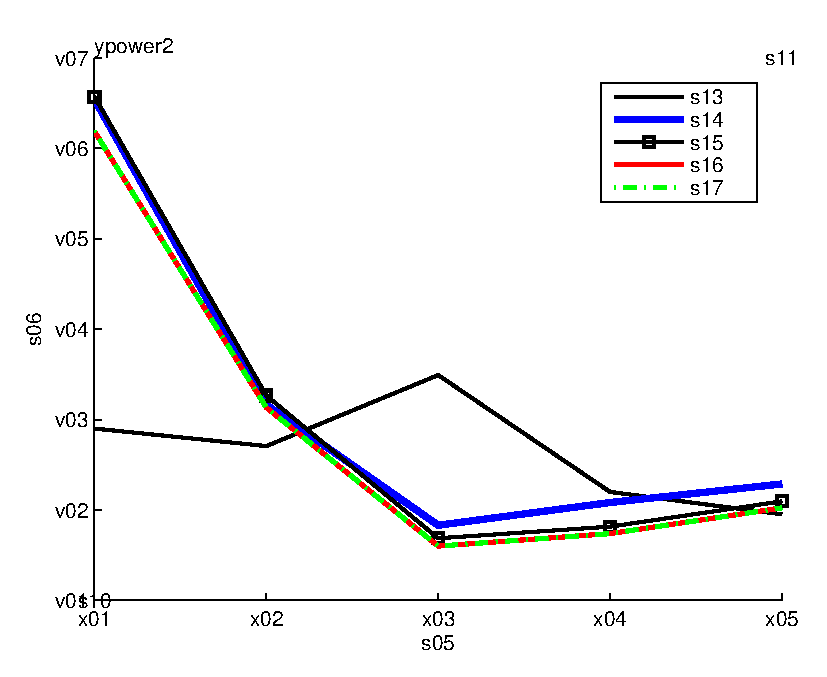
\includegraphics[width=15cm]{mrmse_30.eps}%
\end{psfrags}%
%
% End mrmse_30.tex
\end{document}
% See http://www.mathworks.de/matlabcentral/fileexchange/loadFile.do?objectId=4638
% for recent versions of laprint.m.
%
% created by:           LaPrint version 3.16 (13.9.2004)
% created on:           22-Apr-2014 12:33:29
% eps bounding box:     15 cm x 11.0893 cm
% comment:              
%
\begin{psfrags}%
\psfragscanon%
%
% text strings:
\psfrag{s01}[t][t]{\color[rgb]{0,0,0}\setlength{\tabcolsep}{0pt}\begin{tabular}{c}$\log_2 (M)$\end{tabular}}%
\psfrag{s02}[b][b]{\color[rgb]{0,0,0}\setlength{\tabcolsep}{0pt}\begin{tabular}{c}MRMSE\end{tabular}}%
\psfrag{s06}[][]{\color[rgb]{0,0,0}\setlength{\tabcolsep}{0pt}\begin{tabular}{c} \end{tabular}}%
\psfrag{s07}[][]{\color[rgb]{0,0,0}\setlength{\tabcolsep}{0pt}\begin{tabular}{c} \end{tabular}}%
\psfrag{s08}[l][l]{\color[rgb]{0,0,0}SLF}%
\psfrag{s13}[l][l]{\color[rgb]{0,0,0}EKF}%
\psfrag{s14}[l][l]{\color[rgb]{0,0,0}UKF}%
\psfrag{s15}[l][l]{\color[rgb]{0,0,0}CKF3}%
\psfrag{s16}[l][l]{\color[rgb]{0,0,0}CKF5}%
\psfrag{s17}[l][l]{\color[rgb]{0,0,0}SLF}%
%
% xticklabels:
\psfrag{x01}[t][t]{0}%
\psfrag{x02}[t][t]{0.1}%
\psfrag{x03}[t][t]{0.2}%
\psfrag{x04}[t][t]{0.3}%
\psfrag{x05}[t][t]{0.4}%
\psfrag{x06}[t][t]{0.5}%
\psfrag{x07}[t][t]{0.6}%
\psfrag{x08}[t][t]{0.7}%
\psfrag{x09}[t][t]{0.8}%
\psfrag{x10}[t][t]{0.9}%
\psfrag{x11}[t][t]{1}%
\psfrag{x12}[t][t]{2}%
\psfrag{x13}[t][t]{3}%
\psfrag{x14}[t][t]{4}%
\psfrag{x15}[t][t]{5}%
\psfrag{x16}[t][t]{6}%
%
% yticklabels:
\psfrag{v01}[r][r]{0}%
\psfrag{v02}[r][r]{0.1}%
\psfrag{v03}[r][r]{0.2}%
\psfrag{v04}[r][r]{0.3}%
\psfrag{v05}[r][r]{0.4}%
\psfrag{v06}[r][r]{0.5}%
\psfrag{v07}[r][r]{0.6}%
\psfrag{v08}[r][r]{0.7}%
\psfrag{v09}[r][r]{0.8}%
\psfrag{v10}[r][r]{0.9}%
\psfrag{v11}[r][r]{1}%
\psfrag{v12}[r][r]{4.5}%
\psfrag{v13}[r][r]{5}%
\psfrag{v14}[r][r]{5.5}%
\psfrag{v15}[r][r]{6}%
\psfrag{ypower3}[Bl][Bl]{$\times 10^{-3}$}%
%
% Figure:
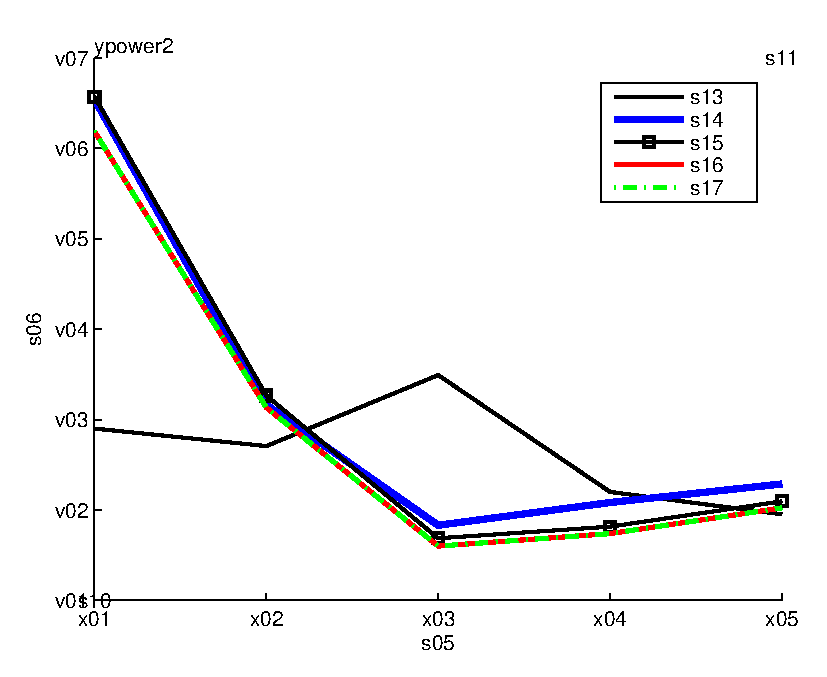
\includegraphics[width=15cm]{mrmse_30.eps}%
\end{psfrags}%
%
% End mrmse_30.tex
\end{document}
% See http://www.mathworks.de/matlabcentral/fileexchange/loadFile.do?objectId=4638
% for recent versions of laprint.m.
%
% created by:           LaPrint version 3.16 (13.9.2004)
% created on:           22-Apr-2014 12:33:29
% eps bounding box:     15 cm x 11.0893 cm
% comment:              
%
\begin{psfrags}%
\psfragscanon%
%
% text strings:
\psfrag{s01}[t][t]{\color[rgb]{0,0,0}\setlength{\tabcolsep}{0pt}\begin{tabular}{c}$\log_2 (M)$\end{tabular}}%
\psfrag{s02}[b][b]{\color[rgb]{0,0,0}\setlength{\tabcolsep}{0pt}\begin{tabular}{c}MRMSE\end{tabular}}%
\psfrag{s06}[][]{\color[rgb]{0,0,0}\setlength{\tabcolsep}{0pt}\begin{tabular}{c} \end{tabular}}%
\psfrag{s07}[][]{\color[rgb]{0,0,0}\setlength{\tabcolsep}{0pt}\begin{tabular}{c} \end{tabular}}%
\psfrag{s08}[l][l]{\color[rgb]{0,0,0}SLF}%
\psfrag{s13}[l][l]{\color[rgb]{0,0,0}EKF}%
\psfrag{s14}[l][l]{\color[rgb]{0,0,0}UKF}%
\psfrag{s15}[l][l]{\color[rgb]{0,0,0}CKF3}%
\psfrag{s16}[l][l]{\color[rgb]{0,0,0}CKF5}%
\psfrag{s17}[l][l]{\color[rgb]{0,0,0}SLF}%
%
% xticklabels:
\psfrag{x01}[t][t]{0}%
\psfrag{x02}[t][t]{0.1}%
\psfrag{x03}[t][t]{0.2}%
\psfrag{x04}[t][t]{0.3}%
\psfrag{x05}[t][t]{0.4}%
\psfrag{x06}[t][t]{0.5}%
\psfrag{x07}[t][t]{0.6}%
\psfrag{x08}[t][t]{0.7}%
\psfrag{x09}[t][t]{0.8}%
\psfrag{x10}[t][t]{0.9}%
\psfrag{x11}[t][t]{1}%
\psfrag{x12}[t][t]{2}%
\psfrag{x13}[t][t]{3}%
\psfrag{x14}[t][t]{4}%
\psfrag{x15}[t][t]{5}%
\psfrag{x16}[t][t]{6}%
%
% yticklabels:
\psfrag{v01}[r][r]{0}%
\psfrag{v02}[r][r]{0.1}%
\psfrag{v03}[r][r]{0.2}%
\psfrag{v04}[r][r]{0.3}%
\psfrag{v05}[r][r]{0.4}%
\psfrag{v06}[r][r]{0.5}%
\psfrag{v07}[r][r]{0.6}%
\psfrag{v08}[r][r]{0.7}%
\psfrag{v09}[r][r]{0.8}%
\psfrag{v10}[r][r]{0.9}%
\psfrag{v11}[r][r]{1}%
\psfrag{v12}[r][r]{4.5}%
\psfrag{v13}[r][r]{5}%
\psfrag{v14}[r][r]{5.5}%
\psfrag{v15}[r][r]{6}%
\psfrag{ypower3}[Bl][Bl]{$\times 10^{-3}$}%
%
% Figure:
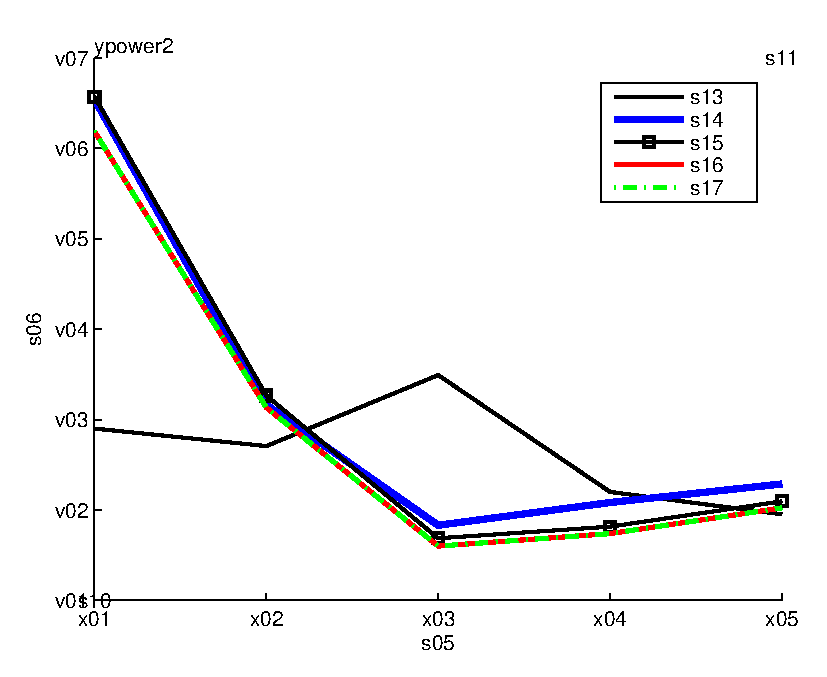
\includegraphics[width=15cm]{mrmse_30.eps}%
\end{psfrags}%
%
% End mrmse_30.tex

\caption{SOC error for $T_s=30$~s as a function of number of integration steps $M$.}
\label{fig:mrmse_30}
\end{figure}

\begin{figure}[p]
\centering
% This file is generated by the MATLAB m-file laprint.m. It can be included
% into LaTeX documents using the packages graphicx, color and psfrag.
% It is accompanied by a postscript file. A sample LaTeX file is:
%    \documentclass{article}\usepackage{graphicx,color,psfrag}
%    \begin{document}% This file is generated by the MATLAB m-file laprint.m. It can be included
% into LaTeX documents using the packages graphicx, color and psfrag.
% It is accompanied by a postscript file. A sample LaTeX file is:
%    \documentclass{article}\usepackage{graphicx,color,psfrag}
%    \begin{document}% This file is generated by the MATLAB m-file laprint.m. It can be included
% into LaTeX documents using the packages graphicx, color and psfrag.
% It is accompanied by a postscript file. A sample LaTeX file is:
%    \documentclass{article}\usepackage{graphicx,color,psfrag}
%    \begin{document}\input{mrmse_det_30}\end{document}
% See http://www.mathworks.de/matlabcentral/fileexchange/loadFile.do?objectId=4638
% for recent versions of laprint.m.
%
% created by:           LaPrint version 3.16 (13.9.2004)
% created on:           09-Apr-2014 02:38:40
% eps bounding box:     15 cm x 11.25 cm
% comment:              
%
\begin{psfrags}%
\psfragscanon%
%
% text strings:
\psfrag{s09}[t][t]{\color[rgb]{0,0,0}\setlength{\tabcolsep}{0pt}\begin{tabular}{c}$\log_2 (M) + 1$\end{tabular}}%
\psfrag{s10}[b][b]{\color[rgb]{0,0,0}\setlength{\tabcolsep}{0pt}\begin{tabular}{c}MRMSE\end{tabular}}%
\psfrag{s14}[][]{\color[rgb]{0,0,0}\setlength{\tabcolsep}{0pt}\begin{tabular}{c} \end{tabular}}%
\psfrag{s15}[][]{\color[rgb]{0,0,0}\setlength{\tabcolsep}{0pt}\begin{tabular}{c} \end{tabular}}%
\psfrag{s16}[l][l]{\color[rgb]{0,0,0}SLF}%
\psfrag{s17}[l][l]{\color[rgb]{0,0,0}EKF}%
\psfrag{s18}[l][l]{\color[rgb]{0,0,0}UKF}%
\psfrag{s19}[l][l]{\color[rgb]{0,0,0}CKF}%
\psfrag{s20}[l][l]{\color[rgb]{0,0,0}SLF}%
%
% xticklabels:
\psfrag{x01}[t][t]{0}%
\psfrag{x02}[t][t]{0.1}%
\psfrag{x03}[t][t]{0.2}%
\psfrag{x04}[t][t]{0.3}%
\psfrag{x05}[t][t]{0.4}%
\psfrag{x06}[t][t]{0.5}%
\psfrag{x07}[t][t]{0.6}%
\psfrag{x08}[t][t]{0.7}%
\psfrag{x09}[t][t]{0.8}%
\psfrag{x10}[t][t]{0.9}%
\psfrag{x11}[t][t]{1}%
\psfrag{x12}[t][t]{2}%
\psfrag{x13}[t][t]{3}%
\psfrag{x14}[t][t]{4}%
\psfrag{x15}[t][t]{5}%
\psfrag{x16}[t][t]{6}%
\psfrag{x17}[t][t]{7}%
\psfrag{x18}[t][t]{8}%
\psfrag{x19}[t][t]{9}%
%
% yticklabels:
\psfrag{v01}[r][r]{0}%
\psfrag{v02}[r][r]{0.1}%
\psfrag{v03}[r][r]{0.2}%
\psfrag{v04}[r][r]{0.3}%
\psfrag{v05}[r][r]{0.4}%
\psfrag{v06}[r][r]{0.5}%
\psfrag{v07}[r][r]{0.6}%
\psfrag{v08}[r][r]{0.7}%
\psfrag{v09}[r][r]{0.8}%
\psfrag{v10}[r][r]{0.9}%
\psfrag{v11}[r][r]{1}%
\psfrag{v12}[r][r]{0}%
\psfrag{v13}[r][r]{0.001}%
\psfrag{v14}[r][r]{0.002}%
\psfrag{v15}[r][r]{0.003}%
\psfrag{v16}[r][r]{0.004}%
\psfrag{v17}[r][r]{0.005}%
\psfrag{v18}[r][r]{0.006}%
\psfrag{v19}[r][r]{0.007}%
\psfrag{v20}[r][r]{0.008}%
\psfrag{v21}[r][r]{0.009}%
\psfrag{v22}[r][r]{0.01}%
%
% Figure:
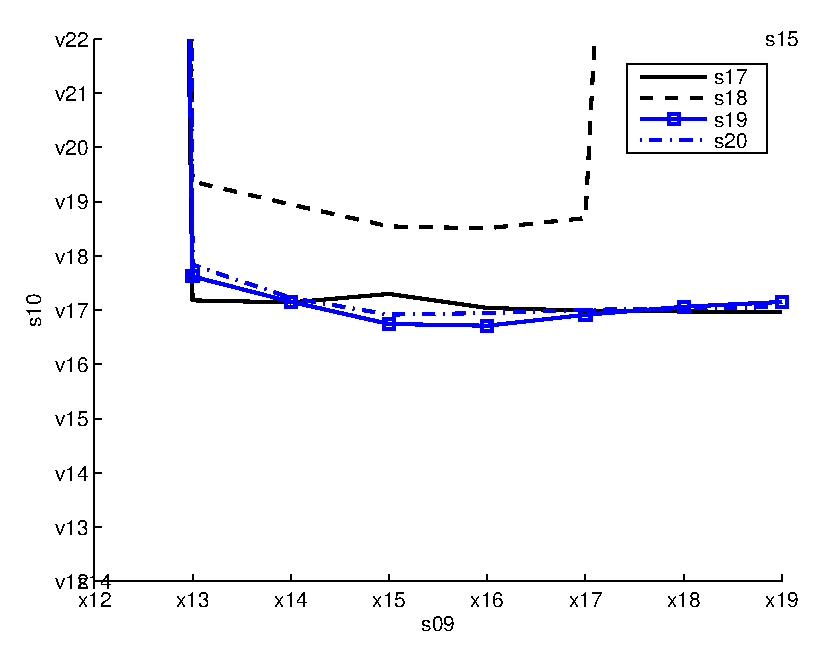
\includegraphics[width=15cm]{mrmse_det_30.eps}%
\end{psfrags}%
%
% End mrmse_det_30.tex
\end{document}
% See http://www.mathworks.de/matlabcentral/fileexchange/loadFile.do?objectId=4638
% for recent versions of laprint.m.
%
% created by:           LaPrint version 3.16 (13.9.2004)
% created on:           09-Apr-2014 02:38:40
% eps bounding box:     15 cm x 11.25 cm
% comment:              
%
\begin{psfrags}%
\psfragscanon%
%
% text strings:
\psfrag{s09}[t][t]{\color[rgb]{0,0,0}\setlength{\tabcolsep}{0pt}\begin{tabular}{c}$\log_2 (M) + 1$\end{tabular}}%
\psfrag{s10}[b][b]{\color[rgb]{0,0,0}\setlength{\tabcolsep}{0pt}\begin{tabular}{c}MRMSE\end{tabular}}%
\psfrag{s14}[][]{\color[rgb]{0,0,0}\setlength{\tabcolsep}{0pt}\begin{tabular}{c} \end{tabular}}%
\psfrag{s15}[][]{\color[rgb]{0,0,0}\setlength{\tabcolsep}{0pt}\begin{tabular}{c} \end{tabular}}%
\psfrag{s16}[l][l]{\color[rgb]{0,0,0}SLF}%
\psfrag{s17}[l][l]{\color[rgb]{0,0,0}EKF}%
\psfrag{s18}[l][l]{\color[rgb]{0,0,0}UKF}%
\psfrag{s19}[l][l]{\color[rgb]{0,0,0}CKF}%
\psfrag{s20}[l][l]{\color[rgb]{0,0,0}SLF}%
%
% xticklabels:
\psfrag{x01}[t][t]{0}%
\psfrag{x02}[t][t]{0.1}%
\psfrag{x03}[t][t]{0.2}%
\psfrag{x04}[t][t]{0.3}%
\psfrag{x05}[t][t]{0.4}%
\psfrag{x06}[t][t]{0.5}%
\psfrag{x07}[t][t]{0.6}%
\psfrag{x08}[t][t]{0.7}%
\psfrag{x09}[t][t]{0.8}%
\psfrag{x10}[t][t]{0.9}%
\psfrag{x11}[t][t]{1}%
\psfrag{x12}[t][t]{2}%
\psfrag{x13}[t][t]{3}%
\psfrag{x14}[t][t]{4}%
\psfrag{x15}[t][t]{5}%
\psfrag{x16}[t][t]{6}%
\psfrag{x17}[t][t]{7}%
\psfrag{x18}[t][t]{8}%
\psfrag{x19}[t][t]{9}%
%
% yticklabels:
\psfrag{v01}[r][r]{0}%
\psfrag{v02}[r][r]{0.1}%
\psfrag{v03}[r][r]{0.2}%
\psfrag{v04}[r][r]{0.3}%
\psfrag{v05}[r][r]{0.4}%
\psfrag{v06}[r][r]{0.5}%
\psfrag{v07}[r][r]{0.6}%
\psfrag{v08}[r][r]{0.7}%
\psfrag{v09}[r][r]{0.8}%
\psfrag{v10}[r][r]{0.9}%
\psfrag{v11}[r][r]{1}%
\psfrag{v12}[r][r]{0}%
\psfrag{v13}[r][r]{0.001}%
\psfrag{v14}[r][r]{0.002}%
\psfrag{v15}[r][r]{0.003}%
\psfrag{v16}[r][r]{0.004}%
\psfrag{v17}[r][r]{0.005}%
\psfrag{v18}[r][r]{0.006}%
\psfrag{v19}[r][r]{0.007}%
\psfrag{v20}[r][r]{0.008}%
\psfrag{v21}[r][r]{0.009}%
\psfrag{v22}[r][r]{0.01}%
%
% Figure:
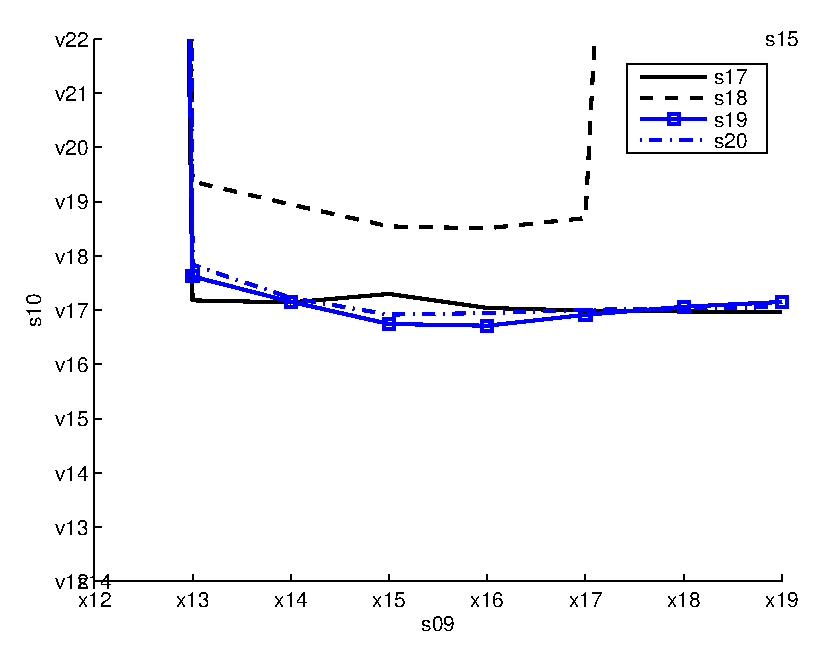
\includegraphics[width=15cm]{mrmse_det_30.eps}%
\end{psfrags}%
%
% End mrmse_det_30.tex
\end{document}
% See http://www.mathworks.de/matlabcentral/fileexchange/loadFile.do?objectId=4638
% for recent versions of laprint.m.
%
% created by:           LaPrint version 3.16 (13.9.2004)
% created on:           09-Apr-2014 02:38:40
% eps bounding box:     15 cm x 11.25 cm
% comment:              
%
\begin{psfrags}%
\psfragscanon%
%
% text strings:
\psfrag{s09}[t][t]{\color[rgb]{0,0,0}\setlength{\tabcolsep}{0pt}\begin{tabular}{c}$\log_2 (M) + 1$\end{tabular}}%
\psfrag{s10}[b][b]{\color[rgb]{0,0,0}\setlength{\tabcolsep}{0pt}\begin{tabular}{c}MRMSE\end{tabular}}%
\psfrag{s14}[][]{\color[rgb]{0,0,0}\setlength{\tabcolsep}{0pt}\begin{tabular}{c} \end{tabular}}%
\psfrag{s15}[][]{\color[rgb]{0,0,0}\setlength{\tabcolsep}{0pt}\begin{tabular}{c} \end{tabular}}%
\psfrag{s16}[l][l]{\color[rgb]{0,0,0}SLF}%
\psfrag{s17}[l][l]{\color[rgb]{0,0,0}EKF}%
\psfrag{s18}[l][l]{\color[rgb]{0,0,0}UKF}%
\psfrag{s19}[l][l]{\color[rgb]{0,0,0}CKF}%
\psfrag{s20}[l][l]{\color[rgb]{0,0,0}SLF}%
%
% xticklabels:
\psfrag{x01}[t][t]{0}%
\psfrag{x02}[t][t]{0.1}%
\psfrag{x03}[t][t]{0.2}%
\psfrag{x04}[t][t]{0.3}%
\psfrag{x05}[t][t]{0.4}%
\psfrag{x06}[t][t]{0.5}%
\psfrag{x07}[t][t]{0.6}%
\psfrag{x08}[t][t]{0.7}%
\psfrag{x09}[t][t]{0.8}%
\psfrag{x10}[t][t]{0.9}%
\psfrag{x11}[t][t]{1}%
\psfrag{x12}[t][t]{2}%
\psfrag{x13}[t][t]{3}%
\psfrag{x14}[t][t]{4}%
\psfrag{x15}[t][t]{5}%
\psfrag{x16}[t][t]{6}%
\psfrag{x17}[t][t]{7}%
\psfrag{x18}[t][t]{8}%
\psfrag{x19}[t][t]{9}%
%
% yticklabels:
\psfrag{v01}[r][r]{0}%
\psfrag{v02}[r][r]{0.1}%
\psfrag{v03}[r][r]{0.2}%
\psfrag{v04}[r][r]{0.3}%
\psfrag{v05}[r][r]{0.4}%
\psfrag{v06}[r][r]{0.5}%
\psfrag{v07}[r][r]{0.6}%
\psfrag{v08}[r][r]{0.7}%
\psfrag{v09}[r][r]{0.8}%
\psfrag{v10}[r][r]{0.9}%
\psfrag{v11}[r][r]{1}%
\psfrag{v12}[r][r]{0}%
\psfrag{v13}[r][r]{0.001}%
\psfrag{v14}[r][r]{0.002}%
\psfrag{v15}[r][r]{0.003}%
\psfrag{v16}[r][r]{0.004}%
\psfrag{v17}[r][r]{0.005}%
\psfrag{v18}[r][r]{0.006}%
\psfrag{v19}[r][r]{0.007}%
\psfrag{v20}[r][r]{0.008}%
\psfrag{v21}[r][r]{0.009}%
\psfrag{v22}[r][r]{0.01}%
%
% Figure:
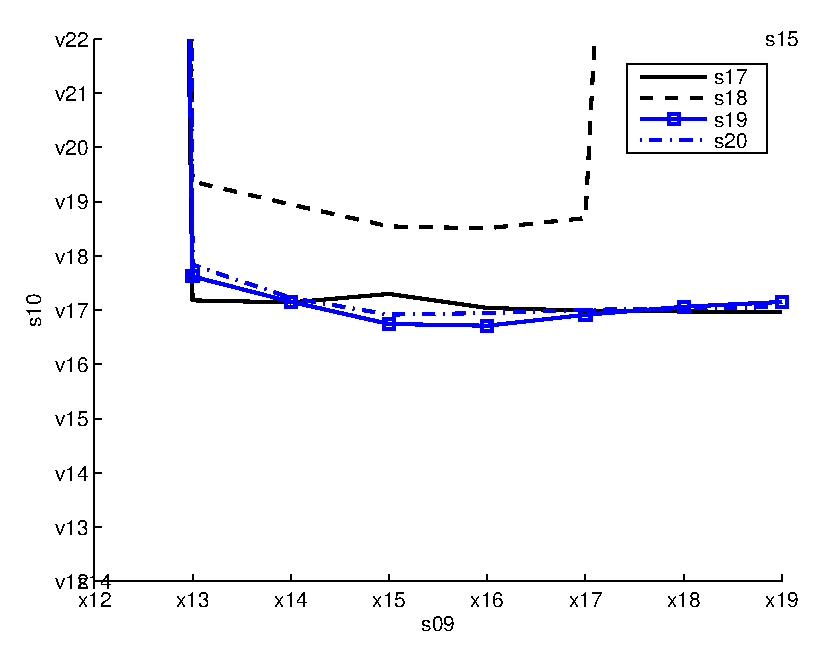
\includegraphics[width=15cm]{mrmse_det_30.eps}%
\end{psfrags}%
%
% End mrmse_det_30.tex

\caption{Detailed view of SOC error for $T_s=30$~s as a function of number of integration steps $M$.}
\label{fig:mrmse_det_30}
\end{figure}

\clearpage

\section{Sampling Period of 150 Seconds}

\begin{table}[h]
\centering
\caption{Number of divergences in 100 Monte Carlo runs for $T_s=150$~s as a function of number of integration steps $M$}
\begin{tabular}{@{}l*{9}{c}@{}}
\toprule
Filter/$M$ & 1   & 2   & 4   & 8   & 16 & 32 & 64 & 128 & 256 \\
\midrule
EKF        & 100 & 100 & 98  & 77  & 0  & 0  & 0  & 0   & 0   \\
UKF        & 100 & 100 & 100 & 100 & 0  & 0  & 0  & 0   & 0   \\
CKF        & 100 & 100 & 100 & 100 & 0  & 0  & 0  & 0   & 0   \\
SLF        & 100 & 100 & 100 & 0   & 0  & 0  & 0  & 0   & 0   \\
\bottomrule
\end{tabular}
\label{tab:div_150}
\end{table}

\begin{table}[h]
\centering
\caption{Filtering time for 100 Monte Carlo runs for $T_s=150$~s as a function of number of integration steps $M$}
\begin{tabular}{@{}lccccccccc@{}}
\toprule
Filter/$M$ & 1      & 2     & 4     & 8     & 16    & 32    & 64    & 128   & 256   \\ \midrule
EKF        & 0.8610 & 2.494 & 7.534 & 8.623 & 4.272 & 8.454 & 17.22 & 34.41 & 68.39 \\
UKF        & 0.8559 & 1.744 & 3.616 & 11.45 & 31.48 & 62.96 & 125.4 & 251.8 & 502.8 \\
CKF        & 0.0310 & 1.621 & 3.204 & 10.11 & 28.04 & 55.88 & 112.4 & 221.2 & 437.9 \\
SLF        & 1.027  & 2.000 & 3.684 & 7.443 & 14.65 & 29.52 & 58.87 & 118.4 & 235.8 \\ \bottomrule
\end{tabular}
\label{tab:time_150}
\end{table}

\clearpage

\begin{figure}[p]
\centering
% This file is generated by the MATLAB m-file laprint.m. It can be included
% into LaTeX documents using the packages graphicx, color and psfrag.
% It is accompanied by a postscript file. A sample LaTeX file is:
%    \documentclass{article}\usepackage{graphicx,color,psfrag}
%    \begin{document}% This file is generated by the MATLAB m-file laprint.m. It can be included
% into LaTeX documents using the packages graphicx, color and psfrag.
% It is accompanied by a postscript file. A sample LaTeX file is:
%    \documentclass{article}\usepackage{graphicx,color,psfrag}
%    \begin{document}% This file is generated by the MATLAB m-file laprint.m. It can be included
% into LaTeX documents using the packages graphicx, color and psfrag.
% It is accompanied by a postscript file. A sample LaTeX file is:
%    \documentclass{article}\usepackage{graphicx,color,psfrag}
%    \begin{document}\input{mrmse_150}\end{document}
% See http://www.mathworks.de/matlabcentral/fileexchange/loadFile.do?objectId=4638
% for recent versions of laprint.m.
%
% created by:           LaPrint version 3.16 (13.9.2004)
% created on:           08-Apr-2014 21:55:04
% eps bounding box:     15 cm x 11.25 cm
% comment:              
%
\begin{psfrags}%
\psfragscanon%
%
% text strings:
\psfrag{s09}[t][t]{\color[rgb]{0,0,0}\setlength{\tabcolsep}{0pt}\begin{tabular}{c}$\log_2 (M) + 1$\end{tabular}}%
\psfrag{s10}[b][b]{\color[rgb]{0,0,0}\setlength{\tabcolsep}{0pt}\begin{tabular}{c}MRMSE\end{tabular}}%
\psfrag{s14}[][]{\color[rgb]{0,0,0}\setlength{\tabcolsep}{0pt}\begin{tabular}{c} \end{tabular}}%
\psfrag{s15}[][]{\color[rgb]{0,0,0}\setlength{\tabcolsep}{0pt}\begin{tabular}{c} \end{tabular}}%
\psfrag{s16}[l][l]{\color[rgb]{0,0,0}SLF}%
\psfrag{s17}[l][l]{\color[rgb]{0,0,0}EKF}%
\psfrag{s18}[l][l]{\color[rgb]{0,0,0}UKF}%
\psfrag{s19}[l][l]{\color[rgb]{0,0,0}CKF}%
\psfrag{s20}[l][l]{\color[rgb]{0,0,0}SLF}%
%
% xticklabels:
\psfrag{x01}[t][t]{0}%
\psfrag{x02}[t][t]{0.1}%
\psfrag{x03}[t][t]{0.2}%
\psfrag{x04}[t][t]{0.3}%
\psfrag{x05}[t][t]{0.4}%
\psfrag{x06}[t][t]{0.5}%
\psfrag{x07}[t][t]{0.6}%
\psfrag{x08}[t][t]{0.7}%
\psfrag{x09}[t][t]{0.8}%
\psfrag{x10}[t][t]{0.9}%
\psfrag{x11}[t][t]{1}%
\psfrag{x12}[t][t]{1}%
\psfrag{x13}[t][t]{2}%
\psfrag{x14}[t][t]{3}%
\psfrag{x15}[t][t]{4}%
\psfrag{x16}[t][t]{5}%
\psfrag{x17}[t][t]{6}%
\psfrag{x18}[t][t]{7}%
\psfrag{x19}[t][t]{8}%
\psfrag{x20}[t][t]{9}%
%
% yticklabels:
\psfrag{v01}[r][r]{0}%
\psfrag{v02}[r][r]{0.1}%
\psfrag{v03}[r][r]{0.2}%
\psfrag{v04}[r][r]{0.3}%
\psfrag{v05}[r][r]{0.4}%
\psfrag{v06}[r][r]{0.5}%
\psfrag{v07}[r][r]{0.6}%
\psfrag{v08}[r][r]{0.7}%
\psfrag{v09}[r][r]{0.8}%
\psfrag{v10}[r][r]{0.9}%
\psfrag{v11}[r][r]{1}%
\psfrag{v12}[r][r]{0}%
\psfrag{v13}[r][r]{0.05}%
\psfrag{v14}[r][r]{0.1}%
\psfrag{v15}[r][r]{0.15}%
\psfrag{v16}[r][r]{0.2}%
\psfrag{v17}[r][r]{0.25}%
\psfrag{v18}[r][r]{0.3}%
\psfrag{v19}[r][r]{0.35}%
\psfrag{v20}[r][r]{0.4}%
\psfrag{v21}[r][r]{0.45}%
\psfrag{v22}[r][r]{0.5}%
%
% Figure:
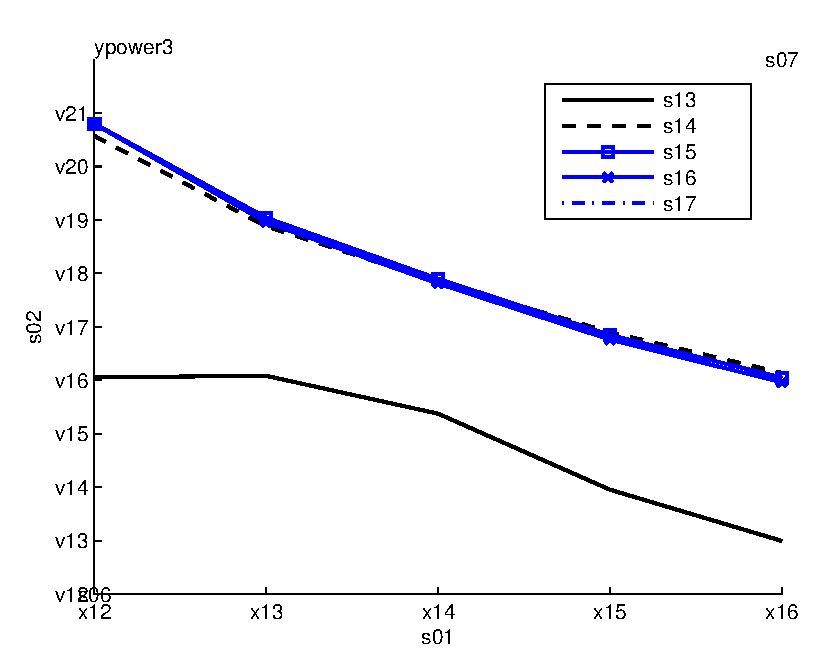
\includegraphics[width=15cm]{mrmse_150.eps}%
\end{psfrags}%
%
% End mrmse_150.tex
\end{document}
% See http://www.mathworks.de/matlabcentral/fileexchange/loadFile.do?objectId=4638
% for recent versions of laprint.m.
%
% created by:           LaPrint version 3.16 (13.9.2004)
% created on:           08-Apr-2014 21:55:04
% eps bounding box:     15 cm x 11.25 cm
% comment:              
%
\begin{psfrags}%
\psfragscanon%
%
% text strings:
\psfrag{s09}[t][t]{\color[rgb]{0,0,0}\setlength{\tabcolsep}{0pt}\begin{tabular}{c}$\log_2 (M) + 1$\end{tabular}}%
\psfrag{s10}[b][b]{\color[rgb]{0,0,0}\setlength{\tabcolsep}{0pt}\begin{tabular}{c}MRMSE\end{tabular}}%
\psfrag{s14}[][]{\color[rgb]{0,0,0}\setlength{\tabcolsep}{0pt}\begin{tabular}{c} \end{tabular}}%
\psfrag{s15}[][]{\color[rgb]{0,0,0}\setlength{\tabcolsep}{0pt}\begin{tabular}{c} \end{tabular}}%
\psfrag{s16}[l][l]{\color[rgb]{0,0,0}SLF}%
\psfrag{s17}[l][l]{\color[rgb]{0,0,0}EKF}%
\psfrag{s18}[l][l]{\color[rgb]{0,0,0}UKF}%
\psfrag{s19}[l][l]{\color[rgb]{0,0,0}CKF}%
\psfrag{s20}[l][l]{\color[rgb]{0,0,0}SLF}%
%
% xticklabels:
\psfrag{x01}[t][t]{0}%
\psfrag{x02}[t][t]{0.1}%
\psfrag{x03}[t][t]{0.2}%
\psfrag{x04}[t][t]{0.3}%
\psfrag{x05}[t][t]{0.4}%
\psfrag{x06}[t][t]{0.5}%
\psfrag{x07}[t][t]{0.6}%
\psfrag{x08}[t][t]{0.7}%
\psfrag{x09}[t][t]{0.8}%
\psfrag{x10}[t][t]{0.9}%
\psfrag{x11}[t][t]{1}%
\psfrag{x12}[t][t]{1}%
\psfrag{x13}[t][t]{2}%
\psfrag{x14}[t][t]{3}%
\psfrag{x15}[t][t]{4}%
\psfrag{x16}[t][t]{5}%
\psfrag{x17}[t][t]{6}%
\psfrag{x18}[t][t]{7}%
\psfrag{x19}[t][t]{8}%
\psfrag{x20}[t][t]{9}%
%
% yticklabels:
\psfrag{v01}[r][r]{0}%
\psfrag{v02}[r][r]{0.1}%
\psfrag{v03}[r][r]{0.2}%
\psfrag{v04}[r][r]{0.3}%
\psfrag{v05}[r][r]{0.4}%
\psfrag{v06}[r][r]{0.5}%
\psfrag{v07}[r][r]{0.6}%
\psfrag{v08}[r][r]{0.7}%
\psfrag{v09}[r][r]{0.8}%
\psfrag{v10}[r][r]{0.9}%
\psfrag{v11}[r][r]{1}%
\psfrag{v12}[r][r]{0}%
\psfrag{v13}[r][r]{0.05}%
\psfrag{v14}[r][r]{0.1}%
\psfrag{v15}[r][r]{0.15}%
\psfrag{v16}[r][r]{0.2}%
\psfrag{v17}[r][r]{0.25}%
\psfrag{v18}[r][r]{0.3}%
\psfrag{v19}[r][r]{0.35}%
\psfrag{v20}[r][r]{0.4}%
\psfrag{v21}[r][r]{0.45}%
\psfrag{v22}[r][r]{0.5}%
%
% Figure:
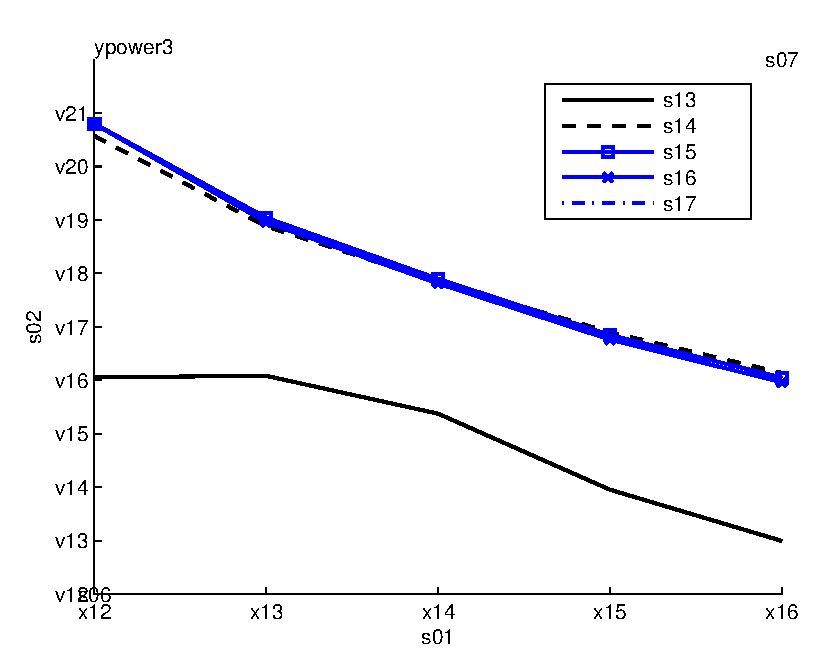
\includegraphics[width=15cm]{mrmse_150.eps}%
\end{psfrags}%
%
% End mrmse_150.tex
\end{document}
% See http://www.mathworks.de/matlabcentral/fileexchange/loadFile.do?objectId=4638
% for recent versions of laprint.m.
%
% created by:           LaPrint version 3.16 (13.9.2004)
% created on:           08-Apr-2014 21:55:04
% eps bounding box:     15 cm x 11.25 cm
% comment:              
%
\begin{psfrags}%
\psfragscanon%
%
% text strings:
\psfrag{s09}[t][t]{\color[rgb]{0,0,0}\setlength{\tabcolsep}{0pt}\begin{tabular}{c}$\log_2 (M) + 1$\end{tabular}}%
\psfrag{s10}[b][b]{\color[rgb]{0,0,0}\setlength{\tabcolsep}{0pt}\begin{tabular}{c}MRMSE\end{tabular}}%
\psfrag{s14}[][]{\color[rgb]{0,0,0}\setlength{\tabcolsep}{0pt}\begin{tabular}{c} \end{tabular}}%
\psfrag{s15}[][]{\color[rgb]{0,0,0}\setlength{\tabcolsep}{0pt}\begin{tabular}{c} \end{tabular}}%
\psfrag{s16}[l][l]{\color[rgb]{0,0,0}SLF}%
\psfrag{s17}[l][l]{\color[rgb]{0,0,0}EKF}%
\psfrag{s18}[l][l]{\color[rgb]{0,0,0}UKF}%
\psfrag{s19}[l][l]{\color[rgb]{0,0,0}CKF}%
\psfrag{s20}[l][l]{\color[rgb]{0,0,0}SLF}%
%
% xticklabels:
\psfrag{x01}[t][t]{0}%
\psfrag{x02}[t][t]{0.1}%
\psfrag{x03}[t][t]{0.2}%
\psfrag{x04}[t][t]{0.3}%
\psfrag{x05}[t][t]{0.4}%
\psfrag{x06}[t][t]{0.5}%
\psfrag{x07}[t][t]{0.6}%
\psfrag{x08}[t][t]{0.7}%
\psfrag{x09}[t][t]{0.8}%
\psfrag{x10}[t][t]{0.9}%
\psfrag{x11}[t][t]{1}%
\psfrag{x12}[t][t]{1}%
\psfrag{x13}[t][t]{2}%
\psfrag{x14}[t][t]{3}%
\psfrag{x15}[t][t]{4}%
\psfrag{x16}[t][t]{5}%
\psfrag{x17}[t][t]{6}%
\psfrag{x18}[t][t]{7}%
\psfrag{x19}[t][t]{8}%
\psfrag{x20}[t][t]{9}%
%
% yticklabels:
\psfrag{v01}[r][r]{0}%
\psfrag{v02}[r][r]{0.1}%
\psfrag{v03}[r][r]{0.2}%
\psfrag{v04}[r][r]{0.3}%
\psfrag{v05}[r][r]{0.4}%
\psfrag{v06}[r][r]{0.5}%
\psfrag{v07}[r][r]{0.6}%
\psfrag{v08}[r][r]{0.7}%
\psfrag{v09}[r][r]{0.8}%
\psfrag{v10}[r][r]{0.9}%
\psfrag{v11}[r][r]{1}%
\psfrag{v12}[r][r]{0}%
\psfrag{v13}[r][r]{0.05}%
\psfrag{v14}[r][r]{0.1}%
\psfrag{v15}[r][r]{0.15}%
\psfrag{v16}[r][r]{0.2}%
\psfrag{v17}[r][r]{0.25}%
\psfrag{v18}[r][r]{0.3}%
\psfrag{v19}[r][r]{0.35}%
\psfrag{v20}[r][r]{0.4}%
\psfrag{v21}[r][r]{0.45}%
\psfrag{v22}[r][r]{0.5}%
%
% Figure:
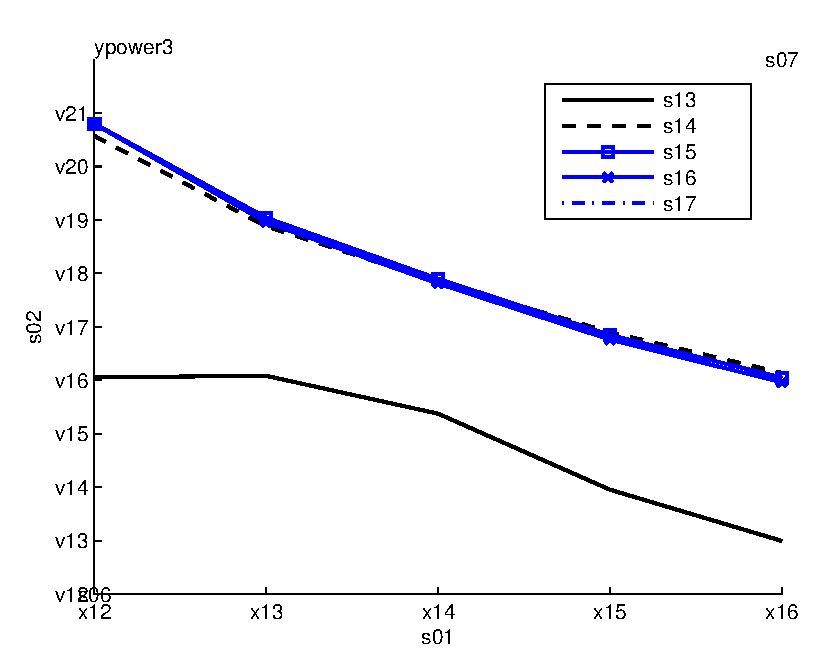
\includegraphics[width=15cm]{mrmse_150.eps}%
\end{psfrags}%
%
% End mrmse_150.tex

\caption{SOC error for $T_s=150$~s as a function of number of integration steps $M$.}
\label{fig:mrmse_150}
\end{figure}

\begin{figure}[p]
\centering
% This file is generated by the MATLAB m-file laprint.m. It can be included
% into LaTeX documents using the packages graphicx, color and psfrag.
% It is accompanied by a postscript file. A sample LaTeX file is:
%    \documentclass{article}\usepackage{graphicx,color,psfrag}
%    \begin{document}% This file is generated by the MATLAB m-file laprint.m. It can be included
% into LaTeX documents using the packages graphicx, color and psfrag.
% It is accompanied by a postscript file. A sample LaTeX file is:
%    \documentclass{article}\usepackage{graphicx,color,psfrag}
%    \begin{document}% This file is generated by the MATLAB m-file laprint.m. It can be included
% into LaTeX documents using the packages graphicx, color and psfrag.
% It is accompanied by a postscript file. A sample LaTeX file is:
%    \documentclass{article}\usepackage{graphicx,color,psfrag}
%    \begin{document}\input{mrmse_det_150}\end{document}
% See http://www.mathworks.de/matlabcentral/fileexchange/loadFile.do?objectId=4638
% for recent versions of laprint.m.
%
% created by:           LaPrint version 3.16 (13.9.2004)
% created on:           09-Apr-2014 02:43:38
% eps bounding box:     15 cm x 11.25 cm
% comment:              
%
\begin{psfrags}%
\psfragscanon%
%
% text strings:
\psfrag{s09}[t][t]{\color[rgb]{0,0,0}\setlength{\tabcolsep}{0pt}\begin{tabular}{c}$\log_2 (M) + 1$\end{tabular}}%
\psfrag{s10}[b][b]{\color[rgb]{0,0,0}\setlength{\tabcolsep}{0pt}\begin{tabular}{c}MRMSE\end{tabular}}%
\psfrag{s14}[][]{\color[rgb]{0,0,0}\setlength{\tabcolsep}{0pt}\begin{tabular}{c} \end{tabular}}%
\psfrag{s15}[][]{\color[rgb]{0,0,0}\setlength{\tabcolsep}{0pt}\begin{tabular}{c} \end{tabular}}%
\psfrag{s16}[l][l]{\color[rgb]{0,0,0}SLF}%
\psfrag{s17}[l][l]{\color[rgb]{0,0,0}EKF}%
\psfrag{s18}[l][l]{\color[rgb]{0,0,0}UKF}%
\psfrag{s19}[l][l]{\color[rgb]{0,0,0}CKF}%
\psfrag{s20}[l][l]{\color[rgb]{0,0,0}SLF}%
%
% xticklabels:
\psfrag{x01}[t][t]{0}%
\psfrag{x02}[t][t]{0.1}%
\psfrag{x03}[t][t]{0.2}%
\psfrag{x04}[t][t]{0.3}%
\psfrag{x05}[t][t]{0.4}%
\psfrag{x06}[t][t]{0.5}%
\psfrag{x07}[t][t]{0.6}%
\psfrag{x08}[t][t]{0.7}%
\psfrag{x09}[t][t]{0.8}%
\psfrag{x10}[t][t]{0.9}%
\psfrag{x11}[t][t]{1}%
\psfrag{x12}[t][t]{4.5}%
\psfrag{x13}[t][t]{5}%
\psfrag{x14}[t][t]{5.5}%
\psfrag{x15}[t][t]{6}%
\psfrag{x16}[t][t]{6.5}%
\psfrag{x17}[t][t]{7}%
\psfrag{x18}[t][t]{7.5}%
\psfrag{x19}[t][t]{8}%
\psfrag{x20}[t][t]{8.5}%
\psfrag{x21}[t][t]{9}%
%
% yticklabels:
\psfrag{v01}[r][r]{0}%
\psfrag{v02}[r][r]{0.1}%
\psfrag{v03}[r][r]{0.2}%
\psfrag{v04}[r][r]{0.3}%
\psfrag{v05}[r][r]{0.4}%
\psfrag{v06}[r][r]{0.5}%
\psfrag{v07}[r][r]{0.6}%
\psfrag{v08}[r][r]{0.7}%
\psfrag{v09}[r][r]{0.8}%
\psfrag{v10}[r][r]{0.9}%
\psfrag{v11}[r][r]{1}%
\psfrag{v12}[r][r]{0}%
\psfrag{v13}[r][r]{0.005}%
\psfrag{v14}[r][r]{0.01}%
\psfrag{v15}[r][r]{0.015}%
%
% Figure:
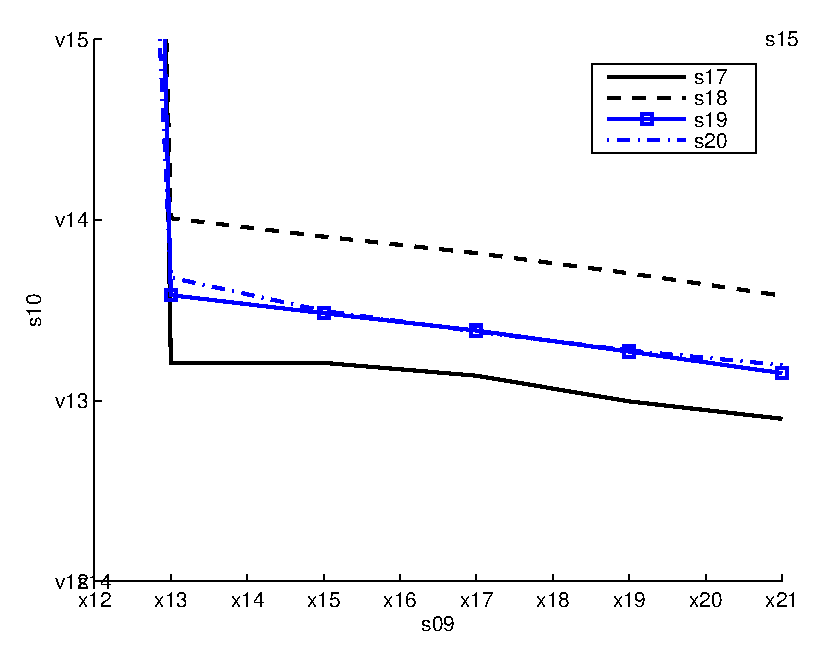
\includegraphics[width=15cm]{mrmse_det_150.eps}%
\end{psfrags}%
%
% End mrmse_det_150.tex
\end{document}
% See http://www.mathworks.de/matlabcentral/fileexchange/loadFile.do?objectId=4638
% for recent versions of laprint.m.
%
% created by:           LaPrint version 3.16 (13.9.2004)
% created on:           09-Apr-2014 02:43:38
% eps bounding box:     15 cm x 11.25 cm
% comment:              
%
\begin{psfrags}%
\psfragscanon%
%
% text strings:
\psfrag{s09}[t][t]{\color[rgb]{0,0,0}\setlength{\tabcolsep}{0pt}\begin{tabular}{c}$\log_2 (M) + 1$\end{tabular}}%
\psfrag{s10}[b][b]{\color[rgb]{0,0,0}\setlength{\tabcolsep}{0pt}\begin{tabular}{c}MRMSE\end{tabular}}%
\psfrag{s14}[][]{\color[rgb]{0,0,0}\setlength{\tabcolsep}{0pt}\begin{tabular}{c} \end{tabular}}%
\psfrag{s15}[][]{\color[rgb]{0,0,0}\setlength{\tabcolsep}{0pt}\begin{tabular}{c} \end{tabular}}%
\psfrag{s16}[l][l]{\color[rgb]{0,0,0}SLF}%
\psfrag{s17}[l][l]{\color[rgb]{0,0,0}EKF}%
\psfrag{s18}[l][l]{\color[rgb]{0,0,0}UKF}%
\psfrag{s19}[l][l]{\color[rgb]{0,0,0}CKF}%
\psfrag{s20}[l][l]{\color[rgb]{0,0,0}SLF}%
%
% xticklabels:
\psfrag{x01}[t][t]{0}%
\psfrag{x02}[t][t]{0.1}%
\psfrag{x03}[t][t]{0.2}%
\psfrag{x04}[t][t]{0.3}%
\psfrag{x05}[t][t]{0.4}%
\psfrag{x06}[t][t]{0.5}%
\psfrag{x07}[t][t]{0.6}%
\psfrag{x08}[t][t]{0.7}%
\psfrag{x09}[t][t]{0.8}%
\psfrag{x10}[t][t]{0.9}%
\psfrag{x11}[t][t]{1}%
\psfrag{x12}[t][t]{4.5}%
\psfrag{x13}[t][t]{5}%
\psfrag{x14}[t][t]{5.5}%
\psfrag{x15}[t][t]{6}%
\psfrag{x16}[t][t]{6.5}%
\psfrag{x17}[t][t]{7}%
\psfrag{x18}[t][t]{7.5}%
\psfrag{x19}[t][t]{8}%
\psfrag{x20}[t][t]{8.5}%
\psfrag{x21}[t][t]{9}%
%
% yticklabels:
\psfrag{v01}[r][r]{0}%
\psfrag{v02}[r][r]{0.1}%
\psfrag{v03}[r][r]{0.2}%
\psfrag{v04}[r][r]{0.3}%
\psfrag{v05}[r][r]{0.4}%
\psfrag{v06}[r][r]{0.5}%
\psfrag{v07}[r][r]{0.6}%
\psfrag{v08}[r][r]{0.7}%
\psfrag{v09}[r][r]{0.8}%
\psfrag{v10}[r][r]{0.9}%
\psfrag{v11}[r][r]{1}%
\psfrag{v12}[r][r]{0}%
\psfrag{v13}[r][r]{0.005}%
\psfrag{v14}[r][r]{0.01}%
\psfrag{v15}[r][r]{0.015}%
%
% Figure:
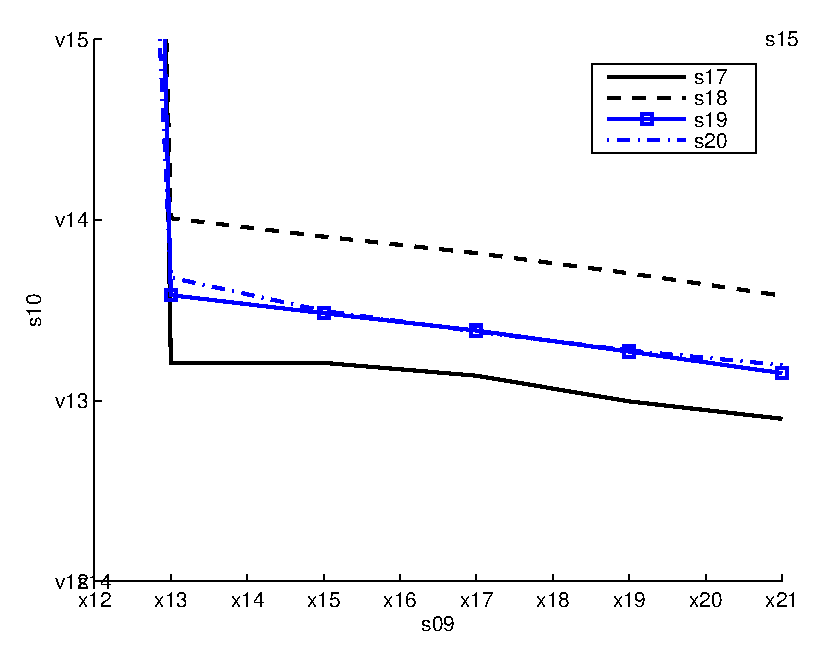
\includegraphics[width=15cm]{mrmse_det_150.eps}%
\end{psfrags}%
%
% End mrmse_det_150.tex
\end{document}
% See http://www.mathworks.de/matlabcentral/fileexchange/loadFile.do?objectId=4638
% for recent versions of laprint.m.
%
% created by:           LaPrint version 3.16 (13.9.2004)
% created on:           09-Apr-2014 02:43:38
% eps bounding box:     15 cm x 11.25 cm
% comment:              
%
\begin{psfrags}%
\psfragscanon%
%
% text strings:
\psfrag{s09}[t][t]{\color[rgb]{0,0,0}\setlength{\tabcolsep}{0pt}\begin{tabular}{c}$\log_2 (M) + 1$\end{tabular}}%
\psfrag{s10}[b][b]{\color[rgb]{0,0,0}\setlength{\tabcolsep}{0pt}\begin{tabular}{c}MRMSE\end{tabular}}%
\psfrag{s14}[][]{\color[rgb]{0,0,0}\setlength{\tabcolsep}{0pt}\begin{tabular}{c} \end{tabular}}%
\psfrag{s15}[][]{\color[rgb]{0,0,0}\setlength{\tabcolsep}{0pt}\begin{tabular}{c} \end{tabular}}%
\psfrag{s16}[l][l]{\color[rgb]{0,0,0}SLF}%
\psfrag{s17}[l][l]{\color[rgb]{0,0,0}EKF}%
\psfrag{s18}[l][l]{\color[rgb]{0,0,0}UKF}%
\psfrag{s19}[l][l]{\color[rgb]{0,0,0}CKF}%
\psfrag{s20}[l][l]{\color[rgb]{0,0,0}SLF}%
%
% xticklabels:
\psfrag{x01}[t][t]{0}%
\psfrag{x02}[t][t]{0.1}%
\psfrag{x03}[t][t]{0.2}%
\psfrag{x04}[t][t]{0.3}%
\psfrag{x05}[t][t]{0.4}%
\psfrag{x06}[t][t]{0.5}%
\psfrag{x07}[t][t]{0.6}%
\psfrag{x08}[t][t]{0.7}%
\psfrag{x09}[t][t]{0.8}%
\psfrag{x10}[t][t]{0.9}%
\psfrag{x11}[t][t]{1}%
\psfrag{x12}[t][t]{4.5}%
\psfrag{x13}[t][t]{5}%
\psfrag{x14}[t][t]{5.5}%
\psfrag{x15}[t][t]{6}%
\psfrag{x16}[t][t]{6.5}%
\psfrag{x17}[t][t]{7}%
\psfrag{x18}[t][t]{7.5}%
\psfrag{x19}[t][t]{8}%
\psfrag{x20}[t][t]{8.5}%
\psfrag{x21}[t][t]{9}%
%
% yticklabels:
\psfrag{v01}[r][r]{0}%
\psfrag{v02}[r][r]{0.1}%
\psfrag{v03}[r][r]{0.2}%
\psfrag{v04}[r][r]{0.3}%
\psfrag{v05}[r][r]{0.4}%
\psfrag{v06}[r][r]{0.5}%
\psfrag{v07}[r][r]{0.6}%
\psfrag{v08}[r][r]{0.7}%
\psfrag{v09}[r][r]{0.8}%
\psfrag{v10}[r][r]{0.9}%
\psfrag{v11}[r][r]{1}%
\psfrag{v12}[r][r]{0}%
\psfrag{v13}[r][r]{0.005}%
\psfrag{v14}[r][r]{0.01}%
\psfrag{v15}[r][r]{0.015}%
%
% Figure:
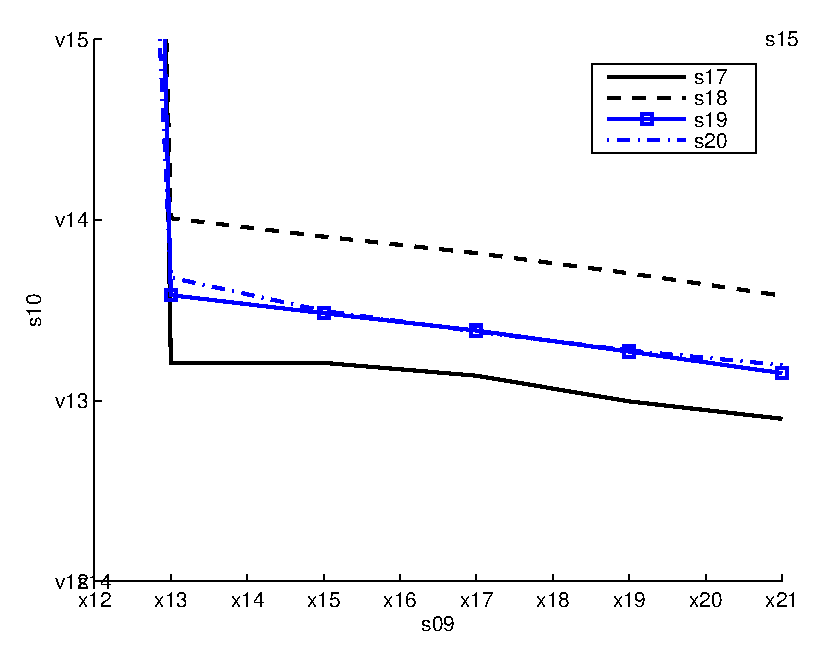
\includegraphics[width=15cm]{mrmse_det_150.eps}%
\end{psfrags}%
%
% End mrmse_det_150.tex

\caption{Detailed view of SOC error for $T_s=150$~s as a function of number of integration steps $M$.}
\label{fig:mrmse_det_150}
\end{figure}

\clearpage

\section{Sampling Period of 300 Seconds}

\begin{table}[h]
\centering
\caption{Number of divergences in 100 Monte Carlo runs for $T_s=300$~s as a function of number of integration steps $M$}
\begin{tabular}{@{}l*{9}{c}@{}}
\toprule
Filter/$M$ & 1   & 2   & 4   & 8   & 16  & 32 & 64 & 128 & 256 \\
\midrule
EKF        & 100 & 100 & 100 & 100 & 68  & 0  & 0  & 0   & 0   \\
UKF        & 100 & 100 & 100 & 100 & 100 & 0  & 0  & 0   & 0   \\
CKF        & 100 & 100 & 100 & 100 & 0   & 0  & 0  & 0   & 0   \\
SLF        & 100 & 100 & 100 & 100 & 0   & 0  & 0  & 0   & 0   \\
\bottomrule
\end{tabular}
\label{tab:div_300}
\end{table}

\begin{table}[h]
\centering
\caption{Filtering time for 100 Monte Carlo runs for $T_s=300$~s as a function of number of integration steps $M$}
\begin{tabular}{@{}lccccccccc@{}}
\toprule
Filter/$M$ & 1      & 2      & 4     & 8     & 16    & 32    & 64    & 128   & 256   \\ \midrule
EKF        & 0.2470 & 0.8910 & 3.572 & 7.913 & 8.174 & 4.451 & 8.755 & 17.62 & 34.38 \\
UKF        & 0.0480 & 0.0480 & 1.543 & 3.477 & 9.372 & 31.64 & 63.17 & 125.9 & 252.0 \\
CKF        & 0.0320 & 0.0640 & 1.535 & 3.061 & 10.28 & 28.27 & 55.80 & 109.7 & 217.9 \\
SLF        & 0.4580 & 1.055  & 1.933 & 3.638 & 7.393 & 14.86 & 29.44 & 58.90 & 117.6 \\ \bottomrule
\end{tabular}
\label{tab:time_300}
\end{table}

\clearpage

\begin{figure}[p]
\centering
% This file is generated by the MATLAB m-file laprint.m. It can be included
% into LaTeX documents using the packages graphicx, color and psfrag.
% It is accompanied by a postscript file. A sample LaTeX file is:
%    \documentclass{article}\usepackage{graphicx,color,psfrag}
%    \begin{document}% This file is generated by the MATLAB m-file laprint.m. It can be included
% into LaTeX documents using the packages graphicx, color and psfrag.
% It is accompanied by a postscript file. A sample LaTeX file is:
%    \documentclass{article}\usepackage{graphicx,color,psfrag}
%    \begin{document}% This file is generated by the MATLAB m-file laprint.m. It can be included
% into LaTeX documents using the packages graphicx, color and psfrag.
% It is accompanied by a postscript file. A sample LaTeX file is:
%    \documentclass{article}\usepackage{graphicx,color,psfrag}
%    \begin{document}\input{mrmse_300}\end{document}
% See http://www.mathworks.de/matlabcentral/fileexchange/loadFile.do?objectId=4638
% for recent versions of laprint.m.
%
% created by:           LaPrint version 3.16 (13.9.2004)
% created on:           08-Apr-2014 21:59:07
% eps bounding box:     15 cm x 11.25 cm
% comment:              
%
\begin{psfrags}%
\psfragscanon%
%
% text strings:
\psfrag{s09}[t][t]{\color[rgb]{0,0,0}\setlength{\tabcolsep}{0pt}\begin{tabular}{c}$\log_2 (M) + 1$\end{tabular}}%
\psfrag{s10}[b][b]{\color[rgb]{0,0,0}\setlength{\tabcolsep}{0pt}\begin{tabular}{c}MRMSE\end{tabular}}%
\psfrag{s14}[][]{\color[rgb]{0,0,0}\setlength{\tabcolsep}{0pt}\begin{tabular}{c} \end{tabular}}%
\psfrag{s15}[][]{\color[rgb]{0,0,0}\setlength{\tabcolsep}{0pt}\begin{tabular}{c} \end{tabular}}%
\psfrag{s16}[l][l]{\color[rgb]{0,0,0}SLF}%
\psfrag{s17}[l][l]{\color[rgb]{0,0,0}EKF}%
\psfrag{s18}[l][l]{\color[rgb]{0,0,0}UKF}%
\psfrag{s19}[l][l]{\color[rgb]{0,0,0}CKF}%
\psfrag{s20}[l][l]{\color[rgb]{0,0,0}SLF}%
%
% xticklabels:
\psfrag{x01}[t][t]{0}%
\psfrag{x02}[t][t]{0.1}%
\psfrag{x03}[t][t]{0.2}%
\psfrag{x04}[t][t]{0.3}%
\psfrag{x05}[t][t]{0.4}%
\psfrag{x06}[t][t]{0.5}%
\psfrag{x07}[t][t]{0.6}%
\psfrag{x08}[t][t]{0.7}%
\psfrag{x09}[t][t]{0.8}%
\psfrag{x10}[t][t]{0.9}%
\psfrag{x11}[t][t]{1}%
\psfrag{x12}[t][t]{1}%
\psfrag{x13}[t][t]{2}%
\psfrag{x14}[t][t]{3}%
\psfrag{x15}[t][t]{4}%
\psfrag{x16}[t][t]{5}%
\psfrag{x17}[t][t]{6}%
\psfrag{x18}[t][t]{7}%
\psfrag{x19}[t][t]{8}%
\psfrag{x20}[t][t]{9}%
%
% yticklabels:
\psfrag{v01}[r][r]{0}%
\psfrag{v02}[r][r]{0.1}%
\psfrag{v03}[r][r]{0.2}%
\psfrag{v04}[r][r]{0.3}%
\psfrag{v05}[r][r]{0.4}%
\psfrag{v06}[r][r]{0.5}%
\psfrag{v07}[r][r]{0.6}%
\psfrag{v08}[r][r]{0.7}%
\psfrag{v09}[r][r]{0.8}%
\psfrag{v10}[r][r]{0.9}%
\psfrag{v11}[r][r]{1}%
\psfrag{v12}[r][r]{0}%
\psfrag{v13}[r][r]{0.05}%
\psfrag{v14}[r][r]{0.1}%
\psfrag{v15}[r][r]{0.15}%
\psfrag{v16}[r][r]{0.2}%
\psfrag{v17}[r][r]{0.25}%
\psfrag{v18}[r][r]{0.3}%
\psfrag{v19}[r][r]{0.35}%
\psfrag{v20}[r][r]{0.4}%
\psfrag{v21}[r][r]{0.45}%
\psfrag{v22}[r][r]{0.5}%
%
% Figure:
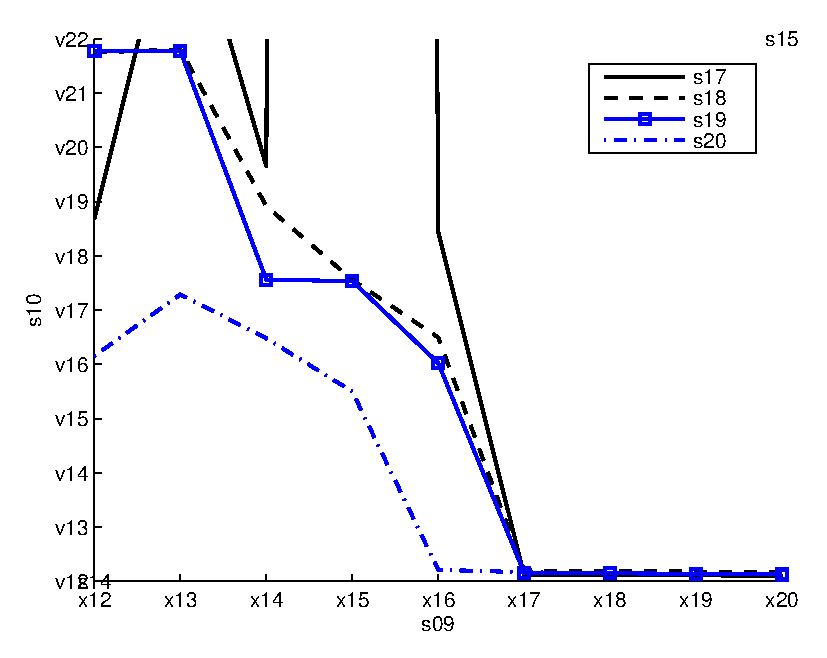
\includegraphics[width=15cm]{mrmse_300.eps}%
\end{psfrags}%
%
% End mrmse_300.tex
\end{document}
% See http://www.mathworks.de/matlabcentral/fileexchange/loadFile.do?objectId=4638
% for recent versions of laprint.m.
%
% created by:           LaPrint version 3.16 (13.9.2004)
% created on:           08-Apr-2014 21:59:07
% eps bounding box:     15 cm x 11.25 cm
% comment:              
%
\begin{psfrags}%
\psfragscanon%
%
% text strings:
\psfrag{s09}[t][t]{\color[rgb]{0,0,0}\setlength{\tabcolsep}{0pt}\begin{tabular}{c}$\log_2 (M) + 1$\end{tabular}}%
\psfrag{s10}[b][b]{\color[rgb]{0,0,0}\setlength{\tabcolsep}{0pt}\begin{tabular}{c}MRMSE\end{tabular}}%
\psfrag{s14}[][]{\color[rgb]{0,0,0}\setlength{\tabcolsep}{0pt}\begin{tabular}{c} \end{tabular}}%
\psfrag{s15}[][]{\color[rgb]{0,0,0}\setlength{\tabcolsep}{0pt}\begin{tabular}{c} \end{tabular}}%
\psfrag{s16}[l][l]{\color[rgb]{0,0,0}SLF}%
\psfrag{s17}[l][l]{\color[rgb]{0,0,0}EKF}%
\psfrag{s18}[l][l]{\color[rgb]{0,0,0}UKF}%
\psfrag{s19}[l][l]{\color[rgb]{0,0,0}CKF}%
\psfrag{s20}[l][l]{\color[rgb]{0,0,0}SLF}%
%
% xticklabels:
\psfrag{x01}[t][t]{0}%
\psfrag{x02}[t][t]{0.1}%
\psfrag{x03}[t][t]{0.2}%
\psfrag{x04}[t][t]{0.3}%
\psfrag{x05}[t][t]{0.4}%
\psfrag{x06}[t][t]{0.5}%
\psfrag{x07}[t][t]{0.6}%
\psfrag{x08}[t][t]{0.7}%
\psfrag{x09}[t][t]{0.8}%
\psfrag{x10}[t][t]{0.9}%
\psfrag{x11}[t][t]{1}%
\psfrag{x12}[t][t]{1}%
\psfrag{x13}[t][t]{2}%
\psfrag{x14}[t][t]{3}%
\psfrag{x15}[t][t]{4}%
\psfrag{x16}[t][t]{5}%
\psfrag{x17}[t][t]{6}%
\psfrag{x18}[t][t]{7}%
\psfrag{x19}[t][t]{8}%
\psfrag{x20}[t][t]{9}%
%
% yticklabels:
\psfrag{v01}[r][r]{0}%
\psfrag{v02}[r][r]{0.1}%
\psfrag{v03}[r][r]{0.2}%
\psfrag{v04}[r][r]{0.3}%
\psfrag{v05}[r][r]{0.4}%
\psfrag{v06}[r][r]{0.5}%
\psfrag{v07}[r][r]{0.6}%
\psfrag{v08}[r][r]{0.7}%
\psfrag{v09}[r][r]{0.8}%
\psfrag{v10}[r][r]{0.9}%
\psfrag{v11}[r][r]{1}%
\psfrag{v12}[r][r]{0}%
\psfrag{v13}[r][r]{0.05}%
\psfrag{v14}[r][r]{0.1}%
\psfrag{v15}[r][r]{0.15}%
\psfrag{v16}[r][r]{0.2}%
\psfrag{v17}[r][r]{0.25}%
\psfrag{v18}[r][r]{0.3}%
\psfrag{v19}[r][r]{0.35}%
\psfrag{v20}[r][r]{0.4}%
\psfrag{v21}[r][r]{0.45}%
\psfrag{v22}[r][r]{0.5}%
%
% Figure:
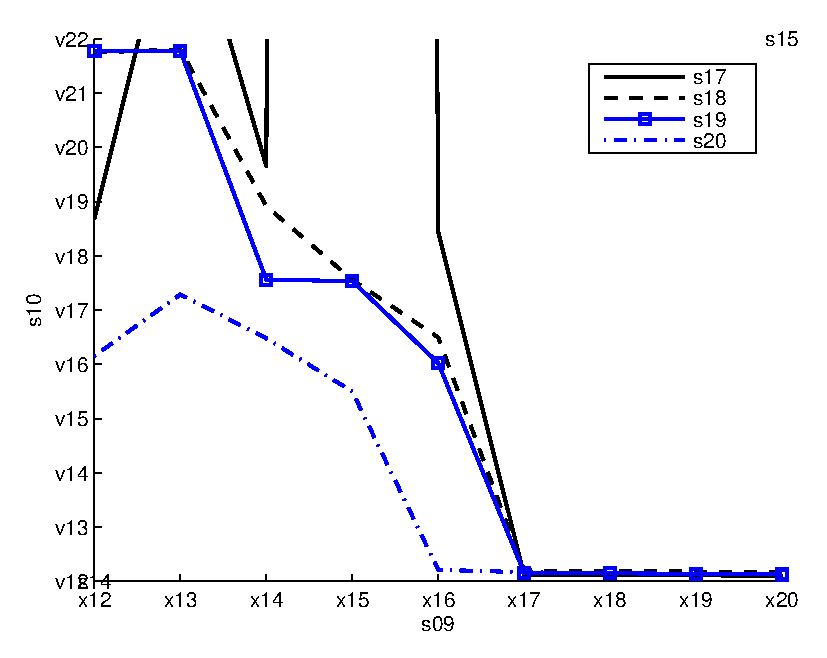
\includegraphics[width=15cm]{mrmse_300.eps}%
\end{psfrags}%
%
% End mrmse_300.tex
\end{document}
% See http://www.mathworks.de/matlabcentral/fileexchange/loadFile.do?objectId=4638
% for recent versions of laprint.m.
%
% created by:           LaPrint version 3.16 (13.9.2004)
% created on:           08-Apr-2014 21:59:07
% eps bounding box:     15 cm x 11.25 cm
% comment:              
%
\begin{psfrags}%
\psfragscanon%
%
% text strings:
\psfrag{s09}[t][t]{\color[rgb]{0,0,0}\setlength{\tabcolsep}{0pt}\begin{tabular}{c}$\log_2 (M) + 1$\end{tabular}}%
\psfrag{s10}[b][b]{\color[rgb]{0,0,0}\setlength{\tabcolsep}{0pt}\begin{tabular}{c}MRMSE\end{tabular}}%
\psfrag{s14}[][]{\color[rgb]{0,0,0}\setlength{\tabcolsep}{0pt}\begin{tabular}{c} \end{tabular}}%
\psfrag{s15}[][]{\color[rgb]{0,0,0}\setlength{\tabcolsep}{0pt}\begin{tabular}{c} \end{tabular}}%
\psfrag{s16}[l][l]{\color[rgb]{0,0,0}SLF}%
\psfrag{s17}[l][l]{\color[rgb]{0,0,0}EKF}%
\psfrag{s18}[l][l]{\color[rgb]{0,0,0}UKF}%
\psfrag{s19}[l][l]{\color[rgb]{0,0,0}CKF}%
\psfrag{s20}[l][l]{\color[rgb]{0,0,0}SLF}%
%
% xticklabels:
\psfrag{x01}[t][t]{0}%
\psfrag{x02}[t][t]{0.1}%
\psfrag{x03}[t][t]{0.2}%
\psfrag{x04}[t][t]{0.3}%
\psfrag{x05}[t][t]{0.4}%
\psfrag{x06}[t][t]{0.5}%
\psfrag{x07}[t][t]{0.6}%
\psfrag{x08}[t][t]{0.7}%
\psfrag{x09}[t][t]{0.8}%
\psfrag{x10}[t][t]{0.9}%
\psfrag{x11}[t][t]{1}%
\psfrag{x12}[t][t]{1}%
\psfrag{x13}[t][t]{2}%
\psfrag{x14}[t][t]{3}%
\psfrag{x15}[t][t]{4}%
\psfrag{x16}[t][t]{5}%
\psfrag{x17}[t][t]{6}%
\psfrag{x18}[t][t]{7}%
\psfrag{x19}[t][t]{8}%
\psfrag{x20}[t][t]{9}%
%
% yticklabels:
\psfrag{v01}[r][r]{0}%
\psfrag{v02}[r][r]{0.1}%
\psfrag{v03}[r][r]{0.2}%
\psfrag{v04}[r][r]{0.3}%
\psfrag{v05}[r][r]{0.4}%
\psfrag{v06}[r][r]{0.5}%
\psfrag{v07}[r][r]{0.6}%
\psfrag{v08}[r][r]{0.7}%
\psfrag{v09}[r][r]{0.8}%
\psfrag{v10}[r][r]{0.9}%
\psfrag{v11}[r][r]{1}%
\psfrag{v12}[r][r]{0}%
\psfrag{v13}[r][r]{0.05}%
\psfrag{v14}[r][r]{0.1}%
\psfrag{v15}[r][r]{0.15}%
\psfrag{v16}[r][r]{0.2}%
\psfrag{v17}[r][r]{0.25}%
\psfrag{v18}[r][r]{0.3}%
\psfrag{v19}[r][r]{0.35}%
\psfrag{v20}[r][r]{0.4}%
\psfrag{v21}[r][r]{0.45}%
\psfrag{v22}[r][r]{0.5}%
%
% Figure:
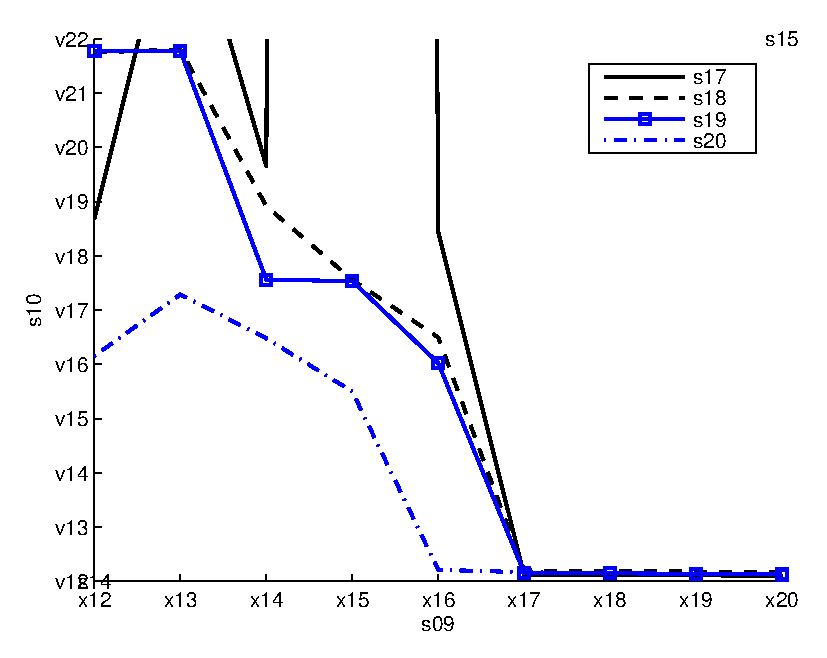
\includegraphics[width=15cm]{mrmse_300.eps}%
\end{psfrags}%
%
% End mrmse_300.tex

\caption{SOC error for $T_s=300$~s as a function of number of integration steps $M$.}
\label{fig:mrmse_300}
\end{figure}

\begin{figure}[p]
\centering
% This file is generated by the MATLAB m-file laprint.m. It can be included
% into LaTeX documents using the packages graphicx, color and psfrag.
% It is accompanied by a postscript file. A sample LaTeX file is:
%    \documentclass{article}\usepackage{graphicx,color,psfrag}
%    \begin{document}% This file is generated by the MATLAB m-file laprint.m. It can be included
% into LaTeX documents using the packages graphicx, color and psfrag.
% It is accompanied by a postscript file. A sample LaTeX file is:
%    \documentclass{article}\usepackage{graphicx,color,psfrag}
%    \begin{document}% This file is generated by the MATLAB m-file laprint.m. It can be included
% into LaTeX documents using the packages graphicx, color and psfrag.
% It is accompanied by a postscript file. A sample LaTeX file is:
%    \documentclass{article}\usepackage{graphicx,color,psfrag}
%    \begin{document}\input{mrmse_det_300}\end{document}
% See http://www.mathworks.de/matlabcentral/fileexchange/loadFile.do?objectId=4638
% for recent versions of laprint.m.
%
% created by:           LaPrint version 3.16 (13.9.2004)
% created on:           09-Apr-2014 02:43:05
% eps bounding box:     15 cm x 11.25 cm
% comment:              
%
\begin{psfrags}%
\psfragscanon%
%
% text strings:
\psfrag{s09}[t][t]{\color[rgb]{0,0,0}\setlength{\tabcolsep}{0pt}\begin{tabular}{c}$\log_2 (M) + 1$\end{tabular}}%
\psfrag{s10}[b][b]{\color[rgb]{0,0,0}\setlength{\tabcolsep}{0pt}\begin{tabular}{c}MRMSE\end{tabular}}%
\psfrag{s14}[][]{\color[rgb]{0,0,0}\setlength{\tabcolsep}{0pt}\begin{tabular}{c} \end{tabular}}%
\psfrag{s15}[][]{\color[rgb]{0,0,0}\setlength{\tabcolsep}{0pt}\begin{tabular}{c} \end{tabular}}%
\psfrag{s16}[l][l]{\color[rgb]{0,0,0}SLF}%
\psfrag{s17}[l][l]{\color[rgb]{0,0,0}EKF}%
\psfrag{s18}[l][l]{\color[rgb]{0,0,0}UKF}%
\psfrag{s19}[l][l]{\color[rgb]{0,0,0}CKF}%
\psfrag{s20}[l][l]{\color[rgb]{0,0,0}SLF}%
%
% xticklabels:
\psfrag{x01}[t][t]{0}%
\psfrag{x02}[t][t]{0.1}%
\psfrag{x03}[t][t]{0.2}%
\psfrag{x04}[t][t]{0.3}%
\psfrag{x05}[t][t]{0.4}%
\psfrag{x06}[t][t]{0.5}%
\psfrag{x07}[t][t]{0.6}%
\psfrag{x08}[t][t]{0.7}%
\psfrag{x09}[t][t]{0.8}%
\psfrag{x10}[t][t]{0.9}%
\psfrag{x11}[t][t]{1}%
\psfrag{x12}[t][t]{4.5}%
\psfrag{x13}[t][t]{5}%
\psfrag{x14}[t][t]{5.5}%
\psfrag{x15}[t][t]{6}%
\psfrag{x16}[t][t]{6.5}%
\psfrag{x17}[t][t]{7}%
\psfrag{x18}[t][t]{7.5}%
\psfrag{x19}[t][t]{8}%
\psfrag{x20}[t][t]{8.5}%
\psfrag{x21}[t][t]{9}%
%
% yticklabels:
\psfrag{v01}[r][r]{0}%
\psfrag{v02}[r][r]{0.1}%
\psfrag{v03}[r][r]{0.2}%
\psfrag{v04}[r][r]{0.3}%
\psfrag{v05}[r][r]{0.4}%
\psfrag{v06}[r][r]{0.5}%
\psfrag{v07}[r][r]{0.6}%
\psfrag{v08}[r][r]{0.7}%
\psfrag{v09}[r][r]{0.8}%
\psfrag{v10}[r][r]{0.9}%
\psfrag{v11}[r][r]{1}%
\psfrag{v12}[r][r]{0}%
\psfrag{v13}[r][r]{0.005}%
\psfrag{v14}[r][r]{0.01}%
\psfrag{v15}[r][r]{0.015}%
%
% Figure:
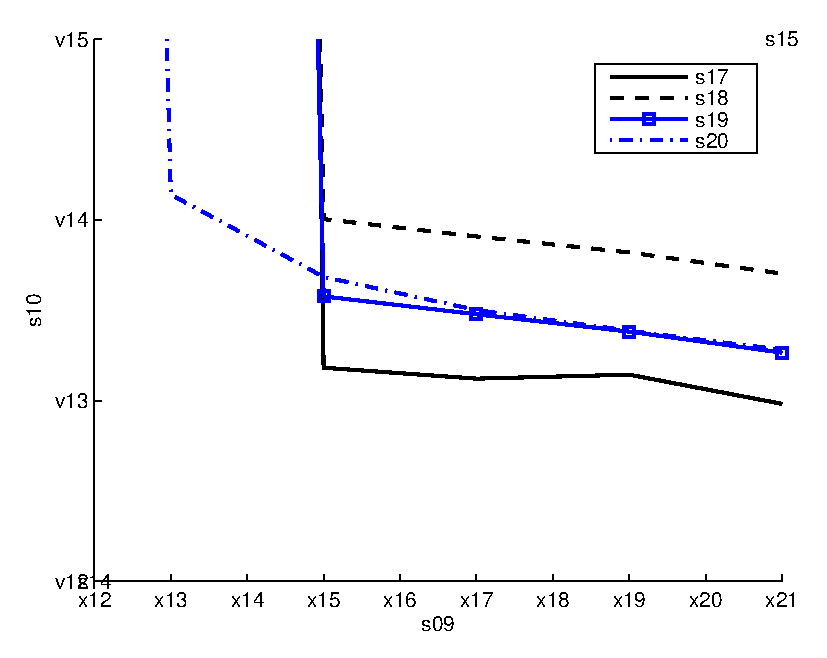
\includegraphics[width=15cm]{mrmse_det_300.eps}%
\end{psfrags}%
%
% End mrmse_det_300.tex
\end{document}
% See http://www.mathworks.de/matlabcentral/fileexchange/loadFile.do?objectId=4638
% for recent versions of laprint.m.
%
% created by:           LaPrint version 3.16 (13.9.2004)
% created on:           09-Apr-2014 02:43:05
% eps bounding box:     15 cm x 11.25 cm
% comment:              
%
\begin{psfrags}%
\psfragscanon%
%
% text strings:
\psfrag{s09}[t][t]{\color[rgb]{0,0,0}\setlength{\tabcolsep}{0pt}\begin{tabular}{c}$\log_2 (M) + 1$\end{tabular}}%
\psfrag{s10}[b][b]{\color[rgb]{0,0,0}\setlength{\tabcolsep}{0pt}\begin{tabular}{c}MRMSE\end{tabular}}%
\psfrag{s14}[][]{\color[rgb]{0,0,0}\setlength{\tabcolsep}{0pt}\begin{tabular}{c} \end{tabular}}%
\psfrag{s15}[][]{\color[rgb]{0,0,0}\setlength{\tabcolsep}{0pt}\begin{tabular}{c} \end{tabular}}%
\psfrag{s16}[l][l]{\color[rgb]{0,0,0}SLF}%
\psfrag{s17}[l][l]{\color[rgb]{0,0,0}EKF}%
\psfrag{s18}[l][l]{\color[rgb]{0,0,0}UKF}%
\psfrag{s19}[l][l]{\color[rgb]{0,0,0}CKF}%
\psfrag{s20}[l][l]{\color[rgb]{0,0,0}SLF}%
%
% xticklabels:
\psfrag{x01}[t][t]{0}%
\psfrag{x02}[t][t]{0.1}%
\psfrag{x03}[t][t]{0.2}%
\psfrag{x04}[t][t]{0.3}%
\psfrag{x05}[t][t]{0.4}%
\psfrag{x06}[t][t]{0.5}%
\psfrag{x07}[t][t]{0.6}%
\psfrag{x08}[t][t]{0.7}%
\psfrag{x09}[t][t]{0.8}%
\psfrag{x10}[t][t]{0.9}%
\psfrag{x11}[t][t]{1}%
\psfrag{x12}[t][t]{4.5}%
\psfrag{x13}[t][t]{5}%
\psfrag{x14}[t][t]{5.5}%
\psfrag{x15}[t][t]{6}%
\psfrag{x16}[t][t]{6.5}%
\psfrag{x17}[t][t]{7}%
\psfrag{x18}[t][t]{7.5}%
\psfrag{x19}[t][t]{8}%
\psfrag{x20}[t][t]{8.5}%
\psfrag{x21}[t][t]{9}%
%
% yticklabels:
\psfrag{v01}[r][r]{0}%
\psfrag{v02}[r][r]{0.1}%
\psfrag{v03}[r][r]{0.2}%
\psfrag{v04}[r][r]{0.3}%
\psfrag{v05}[r][r]{0.4}%
\psfrag{v06}[r][r]{0.5}%
\psfrag{v07}[r][r]{0.6}%
\psfrag{v08}[r][r]{0.7}%
\psfrag{v09}[r][r]{0.8}%
\psfrag{v10}[r][r]{0.9}%
\psfrag{v11}[r][r]{1}%
\psfrag{v12}[r][r]{0}%
\psfrag{v13}[r][r]{0.005}%
\psfrag{v14}[r][r]{0.01}%
\psfrag{v15}[r][r]{0.015}%
%
% Figure:
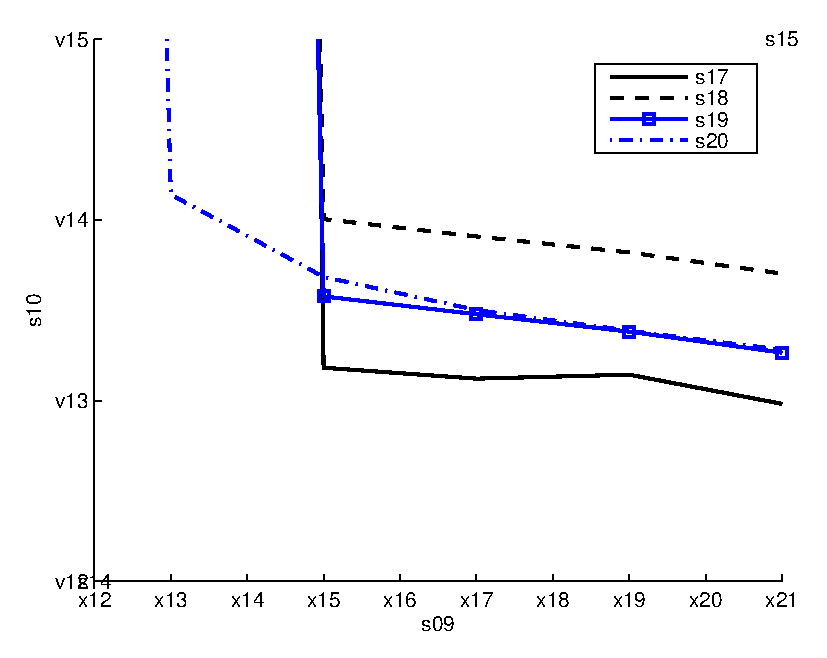
\includegraphics[width=15cm]{mrmse_det_300.eps}%
\end{psfrags}%
%
% End mrmse_det_300.tex
\end{document}
% See http://www.mathworks.de/matlabcentral/fileexchange/loadFile.do?objectId=4638
% for recent versions of laprint.m.
%
% created by:           LaPrint version 3.16 (13.9.2004)
% created on:           09-Apr-2014 02:43:05
% eps bounding box:     15 cm x 11.25 cm
% comment:              
%
\begin{psfrags}%
\psfragscanon%
%
% text strings:
\psfrag{s09}[t][t]{\color[rgb]{0,0,0}\setlength{\tabcolsep}{0pt}\begin{tabular}{c}$\log_2 (M) + 1$\end{tabular}}%
\psfrag{s10}[b][b]{\color[rgb]{0,0,0}\setlength{\tabcolsep}{0pt}\begin{tabular}{c}MRMSE\end{tabular}}%
\psfrag{s14}[][]{\color[rgb]{0,0,0}\setlength{\tabcolsep}{0pt}\begin{tabular}{c} \end{tabular}}%
\psfrag{s15}[][]{\color[rgb]{0,0,0}\setlength{\tabcolsep}{0pt}\begin{tabular}{c} \end{tabular}}%
\psfrag{s16}[l][l]{\color[rgb]{0,0,0}SLF}%
\psfrag{s17}[l][l]{\color[rgb]{0,0,0}EKF}%
\psfrag{s18}[l][l]{\color[rgb]{0,0,0}UKF}%
\psfrag{s19}[l][l]{\color[rgb]{0,0,0}CKF}%
\psfrag{s20}[l][l]{\color[rgb]{0,0,0}SLF}%
%
% xticklabels:
\psfrag{x01}[t][t]{0}%
\psfrag{x02}[t][t]{0.1}%
\psfrag{x03}[t][t]{0.2}%
\psfrag{x04}[t][t]{0.3}%
\psfrag{x05}[t][t]{0.4}%
\psfrag{x06}[t][t]{0.5}%
\psfrag{x07}[t][t]{0.6}%
\psfrag{x08}[t][t]{0.7}%
\psfrag{x09}[t][t]{0.8}%
\psfrag{x10}[t][t]{0.9}%
\psfrag{x11}[t][t]{1}%
\psfrag{x12}[t][t]{4.5}%
\psfrag{x13}[t][t]{5}%
\psfrag{x14}[t][t]{5.5}%
\psfrag{x15}[t][t]{6}%
\psfrag{x16}[t][t]{6.5}%
\psfrag{x17}[t][t]{7}%
\psfrag{x18}[t][t]{7.5}%
\psfrag{x19}[t][t]{8}%
\psfrag{x20}[t][t]{8.5}%
\psfrag{x21}[t][t]{9}%
%
% yticklabels:
\psfrag{v01}[r][r]{0}%
\psfrag{v02}[r][r]{0.1}%
\psfrag{v03}[r][r]{0.2}%
\psfrag{v04}[r][r]{0.3}%
\psfrag{v05}[r][r]{0.4}%
\psfrag{v06}[r][r]{0.5}%
\psfrag{v07}[r][r]{0.6}%
\psfrag{v08}[r][r]{0.7}%
\psfrag{v09}[r][r]{0.8}%
\psfrag{v10}[r][r]{0.9}%
\psfrag{v11}[r][r]{1}%
\psfrag{v12}[r][r]{0}%
\psfrag{v13}[r][r]{0.005}%
\psfrag{v14}[r][r]{0.01}%
\psfrag{v15}[r][r]{0.015}%
%
% Figure:
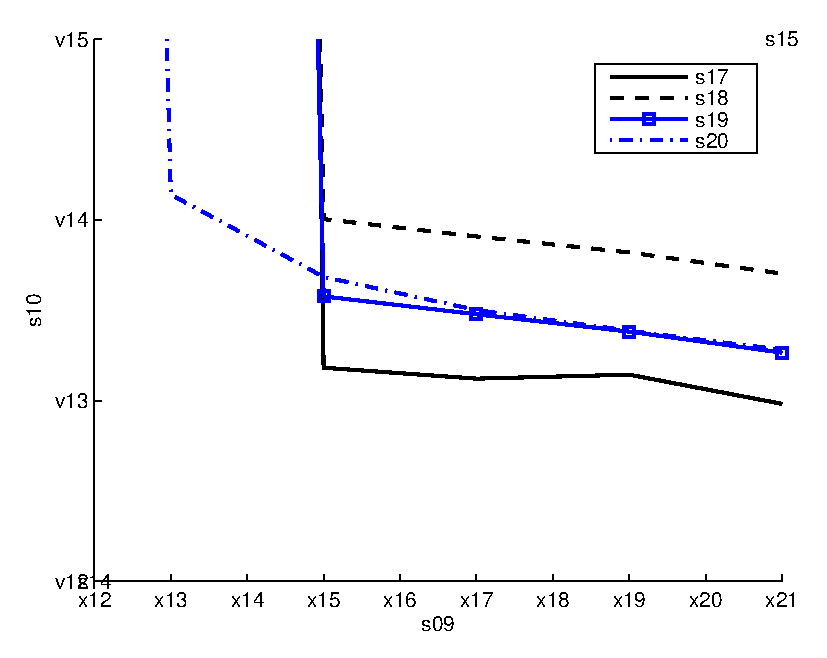
\includegraphics[width=15cm]{mrmse_det_300.eps}%
\end{psfrags}%
%
% End mrmse_det_300.tex

\caption{Detailed view of SOC error for $T_s=300$~s as a function of number of integration steps $M$.}
\label{fig:mrmse_det_300}
\end{figure}

\end{document}
